
% this file is called up by thesis.tex
% content in this file will be fed into the main document

%: ----------------------- introduction file header -----------------------
\chapter{Explainable Topic-based Associations}\label{ch:explainability}

\graphicspath{{explainability/figures/}}

% -------------------------------------------------------------
% -- Explainability
% -------------------------------------------------------------

As stated in Chapter \ref{ch:hypothesis}, one of our hypotheses aims to determine whether it is possible to semantically relate texts taking into account their most relevant topics (H1.2). In particular, our goal is to determine whether two documents can be related by identifying their most representative topics.

However, as seen in Section \ref{sec:topic-explainability}, interpreting how documents are related from their topic distributions is hard when using density-based measures (e.g. distance equals to 0.74 or 0.76). The same pair of documents may vary their distance from each other when using topic models with different dimensions to represent them, as shown in figure \ref{fig:topic_distances}. High dimensional models create more specific topics than models with fewer dimensions, and this topic specificity influences the way in which topic distributions are related, and consequently how documents can be related. 

In order to better understand the relations derived from topic distributions, Section \ref{sec:topic-relations} compares scientific articles from their representations based on full-content, abstracts (i.e manual summaries), or summaries created automatically. Two types of metrics are considered: (i) \textit{internal-representativeness}, focused on describing the content, and \textit{external-representativeness}, focused on discovering relations \citep{Badenes-Olmedo2017c}.    

In Section \ref{sec:topic-clustering}, once we know how the topics are used to represent and relate texts, we propose a new topic-based annotation based only on the most representative topics, and a new distance measure that takes advantage of these representations \citep{Badenes-Olmedo2017b}. The main goal is not only to cluster texts through their most relevant topics, but also to facilitate the interpretation of their relations. 


\section{Topic-based Relations}
\label{sec:topic-relations}

This section studies the ability of topic distributions to capture the representativeness of a text through the relations that can be derived from it. In particular, it examines the performance offered by topic-based representations to describe scientific articles from their full-texts compared to representations based on summaries (e.g. \textit{abstract}). The objective is twofold, to analyze comparisons based on topic distributions on the one hand, and to identify strengths and weaknesses when using \textit{abstracts} to compare scientific articles on the other hand . Two novel measures are proposed based on the capability of the summary to substitute the original paper (Figure \ref{fig:representativeness}): (1) \textit{internal-representativeness}, which evaluates how well the summary represents the original full-text and (2) \textit{external-representativeness}, which evaluates the summary according to how the summary is able to produce a  set of related texts that are similar to what the original full-text has triggered.

Some studies \citep{Westergaard2017, Sciences2016} have shown that text mining of full research articles give consistently better results than using only their corresponding abstracts. Given the size limitations and concise nature of abstracts, they often omit descriptions or results that are considered to be less relevant but still are important in certain Information Retrieval tasks. Thus, when other researchers cite a particular paper, 20\% of the keywords that they mention are not present in the abstract \citep{Divoli2012}.

\begin{figure}[!htbp]
\centering
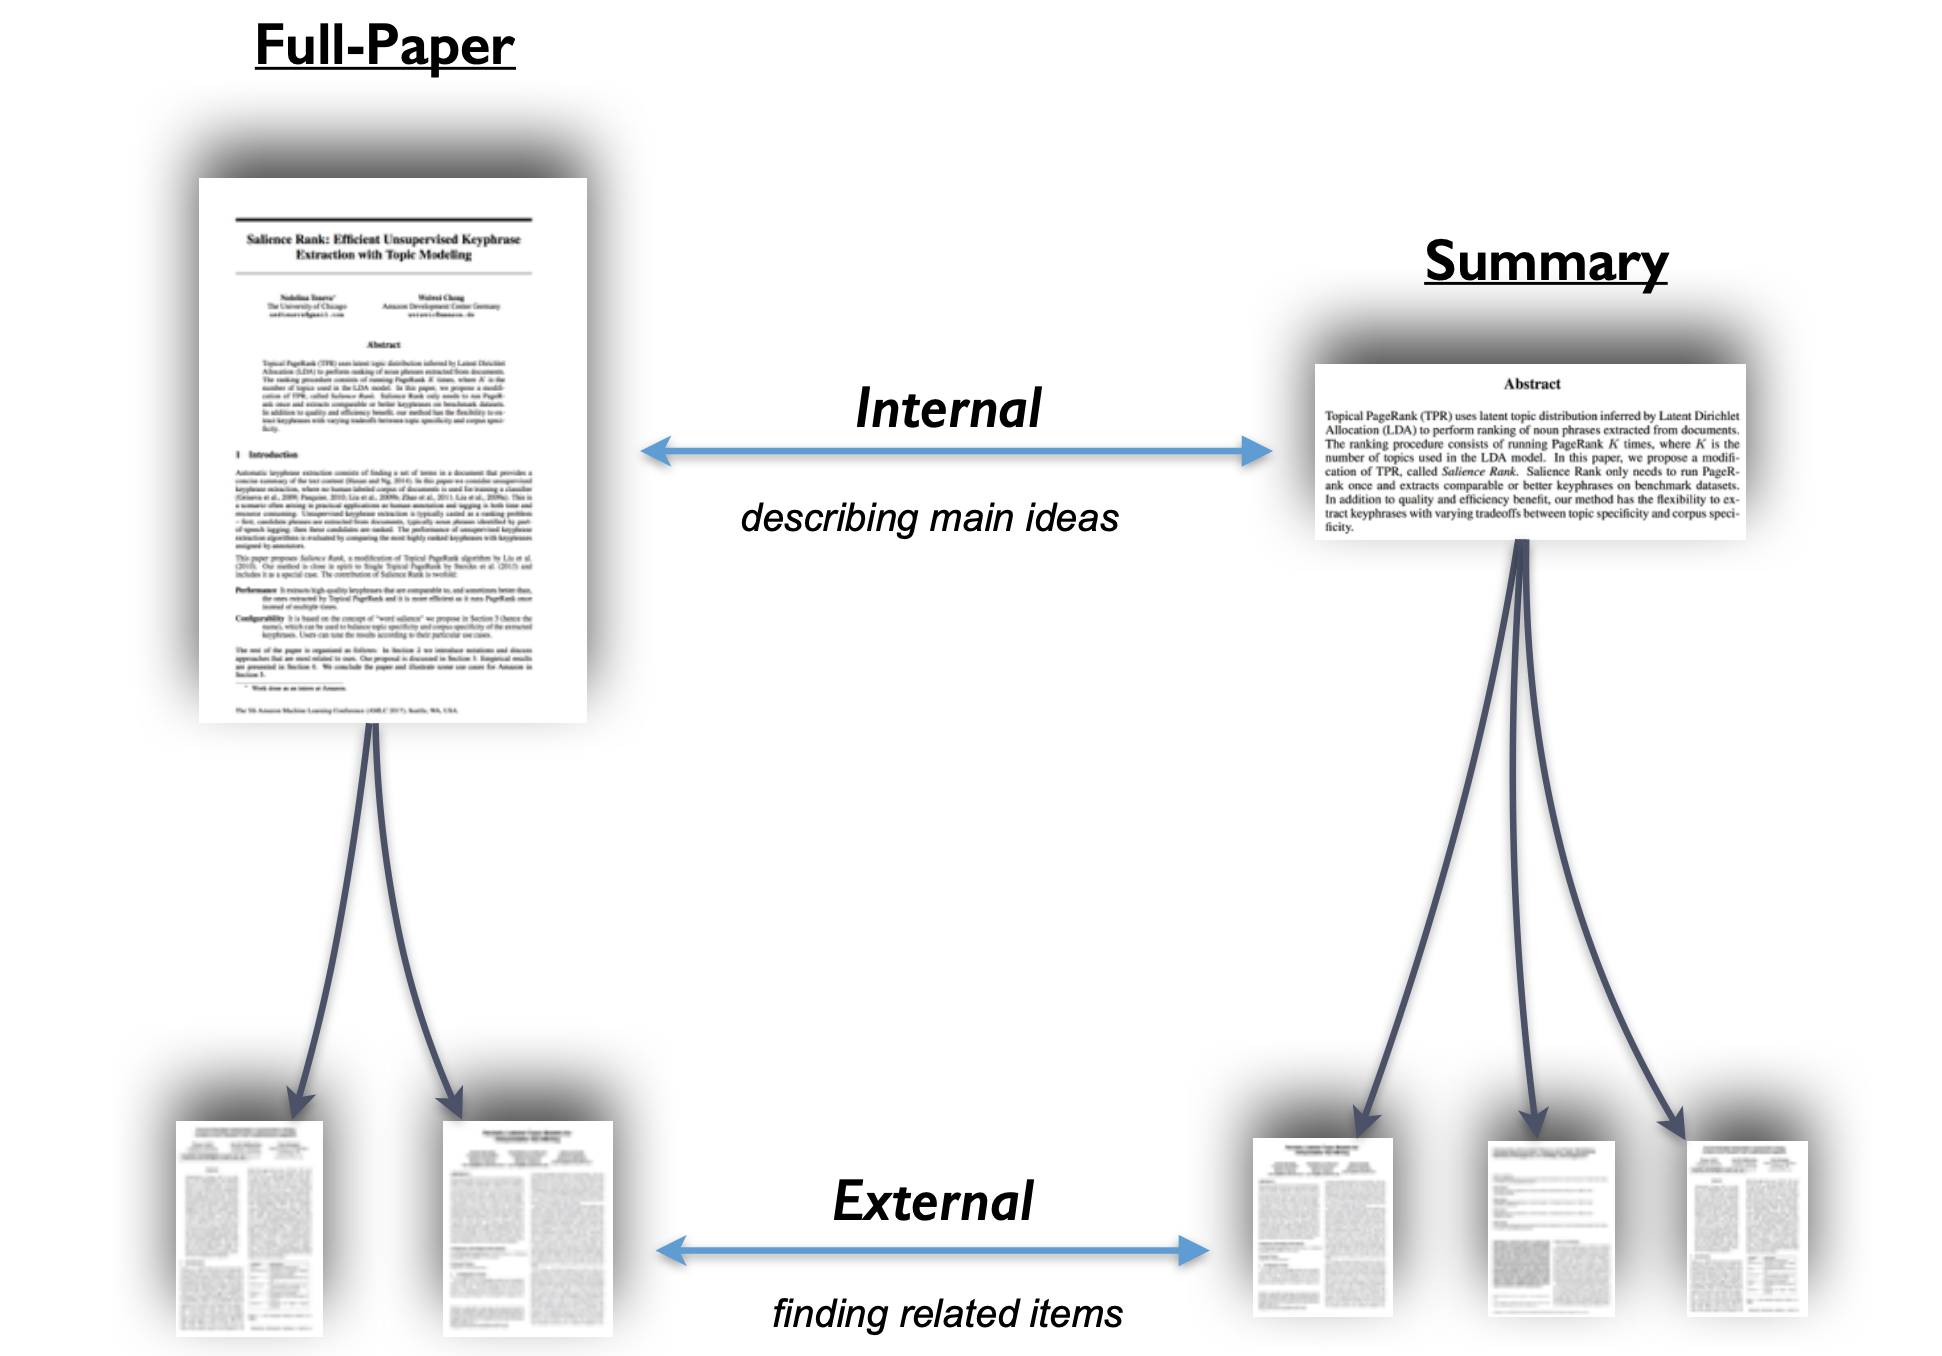
\includegraphics[scale=0.24]{internal-external.png}
\caption{Internal and External Representativeness. }
\label{fig:representativeness}
\end{figure}


An analysis about the \textit{representativeness} of research article summaries based on topic distributions is presented in this section, considering those based exclusively on abstracts and those based on their discursive structure (\textit{approach}, \textit{challenge}, \textit{background}, \textit{outcomes} and \textit{future work})\citep{SimoneTeufel2010}. The \textit{representativeness} of a summary with respect to the original full-text is assumed as the degree of relation with the original one (\textit{internal-representativeness}), along with the capacity of mimicking the full text when finding related items (\textit{external-representativeness}). In order to quantify this notion of internal-external representativeness, a probabilistic topic model is trained to have a vectorial representation of each text retrieved from a paper: full content-based and summary-based (Figure \ref{fig:representativeness}). The vectorial representations of full-papers is used to measure the distance between them and those derived from abstract or summaries (\textit{internal-representativeness}), and also to find similar documents (\textit{external- representativeness}) based on the distance between their vectorial representations. An upper distance threshold is specified to filter less similar pairs and compose a set of related papers for each paper. Then, a comparison in terms of \textit{precision} and \textit{recall} is performed between sets obtained by only using the vectorial representation of full-papers, against sets produced by using other kind of summaries.

\subsection{Research Articles Summaries}
\label{sec:annotator}
Some approaches have been proposed to summarize scientific articles \citep{Cohan2015} taking advantage of the citation context and the document discourse model. We have used the scientific discourse annotator proposed by \citep{Ronzano2015} to automatically create summaries from research papers by classifying each sentence as belonging to one of the following scientific discourse categories: \textit{approach}, \textit{challenge},  \textit{background}, \textit{outcomes} and \textit{future work}. These categories were identified from the schemata proposed by \citep{Teufel2009} with an original purpose of characterizing the content of Computer Graphics papers. 

The annotator is based on a Support Vector Machine classifier that combines both lexical and syntactic features to model each sentence in a paper. The tool\footnote{http://backingdata.org/dri/library/} was integrated in our \textit{librAIry} framework through the \textit{Rhetoric Module}\footnote{https://github.com/librairy/annotator-rhetoric} to automatically annotate research papers with their rhetorical content.

\begin{figure}[!htbp]
\centering
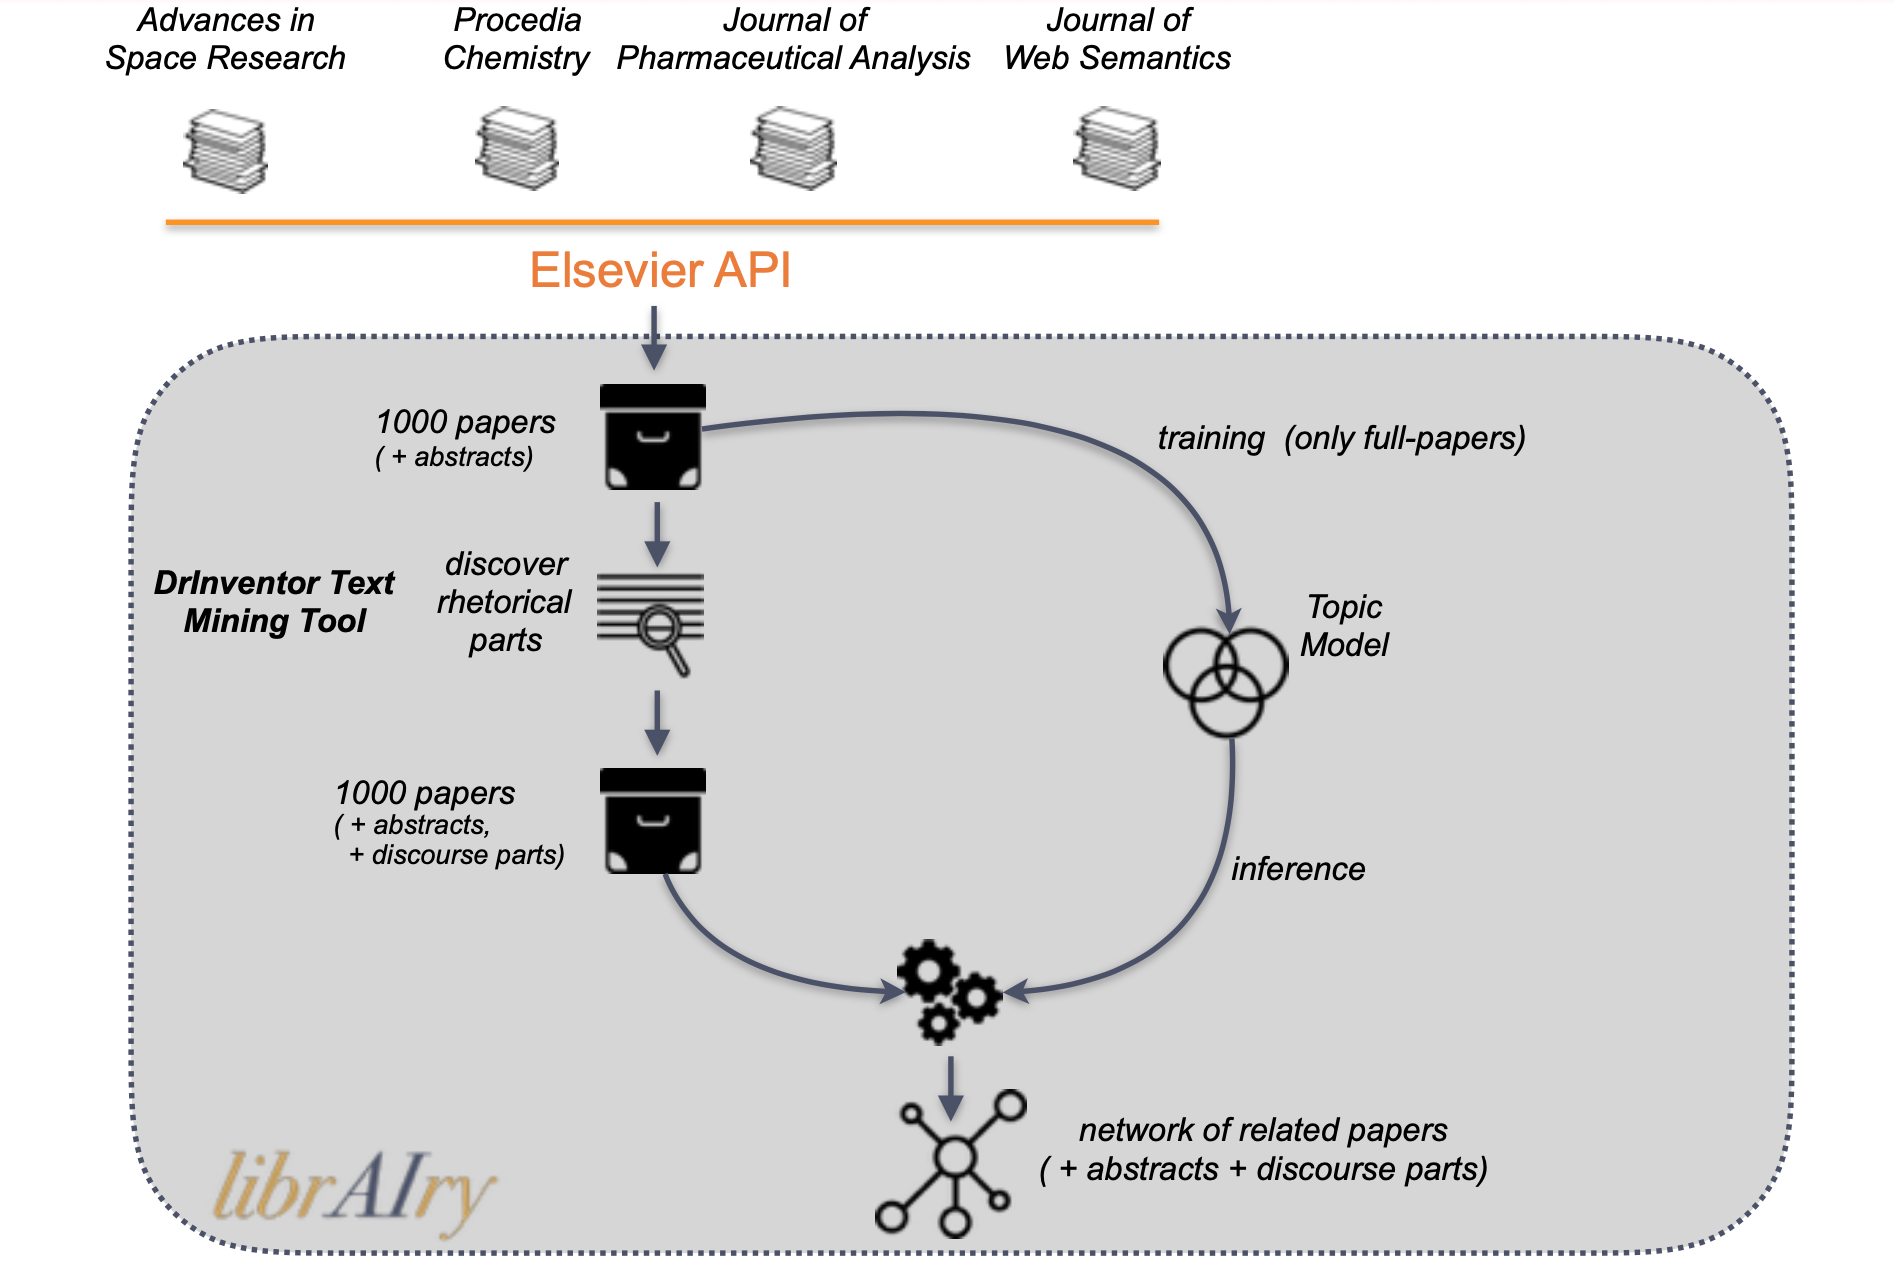
\includegraphics[scale=0.40]{similarity-experiment.png}
\caption{Experiment to analyze the ability of topic-based representations to create relations from summaries \textit{vs} full-texts. }
\label{fig:similarity-experiment}
\end{figure}

\subsection{Feature Vectors}
\label{sec:topicmodel}
A representational model is required not only to measure distances between text fragments but, more importantly, to help to understand the differences in their content. As seen in Section \ref{sec:topic-explainability}, topic models are widely used to uncover the latent semantic structure from text corpora. In particular, Probabilistic Topic Models represent documents as a mixture of topics, where topics are probability distributions over words. Latent Dirichlet Allocation (LDA)\citep{Blei2003} is the simplest \textit{generative} topic model that makes it possible to characterize documents not previously used during the training task. This is a key feature for our evaluations because, although the model used for the experiments will be trained from the full-content of papers, it will be also used to describe the texts summaries.

Thus, we have used a LDA model to describe the inherent topic distribution of papers in the corpus. Some hyper-parameters need to be estimated: the \textit{number of topics (k)}, the  concentration parameter ($\alpha$) for the prior placed on documents' distributions over topics and the concentration parameter ($\beta$) for the prior placed on topics’ distributions over terms. Since the target of this experiment is not to evaluate the quality of the representational model, but to compare their topic distributions, we accepted as valid values those widely used in the literature: $\alpha=0.1$, $\beta=0.1$ , and $k=2*\sqrt{n/2}=44$ where $n$ is the size of the corpus.



\subsection{Similarity Measure}
Feature vectors in Topic Models are topic distributions expressed as vectors of probabilities. Hence we opt for \textit{Jensen-Shannon divergence} (JS) (See Section \ref{sec:related-work})  instead of the commonly used \textit{Kullback-Liebler divergence} (KL). The reason for this is that KL is not defined when a topic distribution is zero and is not symmetric, what does not fit well with semantic similarity measures which in general are symmetric \citep{Rus2013}. JS considers the average of the distributions as follows :

\begin{equation}
JS(p,q) = \sum\limits_{i=1}^T p_{i}*\log \frac{2*p_{i}}{p_{i}+q_{i}}  +  \sum\limits_{i=1}^T q_{i}*\log \frac{2*q_{i}}{q_{i}+p_{i}}
\label{eq:jsd}
\end{equation}
where  $T$ is the number of topics and $p,q$ are the topics distributions.

And the \textit{similarity measure} used in our analysis is based on the JS transformed into a similarity measure as follows \citep{Dagan1998} :

\begin{equation}
similarity(D_i , D_j) = 10^{- JS(p,q)}
\label{eq:simcontent}
\end{equation}
where  $D_i,D_j$ are the documents and $p,q$ the topics distributions of each of them.

\subsection{Evaluation}
\label{sec:topic-relevance-experiments}

The corpus used in the experiments was created by combining journals in different scientific domains such as \textit{Advances in Space Research}, \textit{Procedia Chemistry}, \textit{Journal of Pharmaceutical Analysis} and \textit{Journal of Web Semantics} (Figure \ref{fig:similarity-experiment}). In total 1,000 papers were added, 250 from each journal. Both the abstract and the \textit{full-content} of these documents were directly retrieved from the Elsevier API \footnote{https://dev.elsevier.com} by using our \textit{Harvester module} \footnote{https://github.com/librairy/harvester-elsevier}. The code used to perform the analysis along with the results obtained are publicly available\footnote{https://github.com/librairy/study-semantic-similarity}.

Since the annotation process to automatically discover the rhetorical parts of a research paper (Section ~\ref{sec:annotator}) is sensitive to the structure of the phrases that are used when writing the text, only $20\%$ of papers in the corpus could be fully annotated with all the fragments considered. In fact, these categories are not present in the same proportion in the corpus: \textit{approach} ($90\%$), \textit{background} ($78\%$), \textit{outcome} ($73\%$), \textit{challenge} ($57\%$) and \textit{future work} ($21\%$)

\subsubsection{Internal Representativeness}

The \textit{internal-representativeness} of a text measures the similarity of a summary against the original full-text. This measure is based on the JS between the topic distribution of each of them. 

\begin{figure}[!htbp]
  \center
  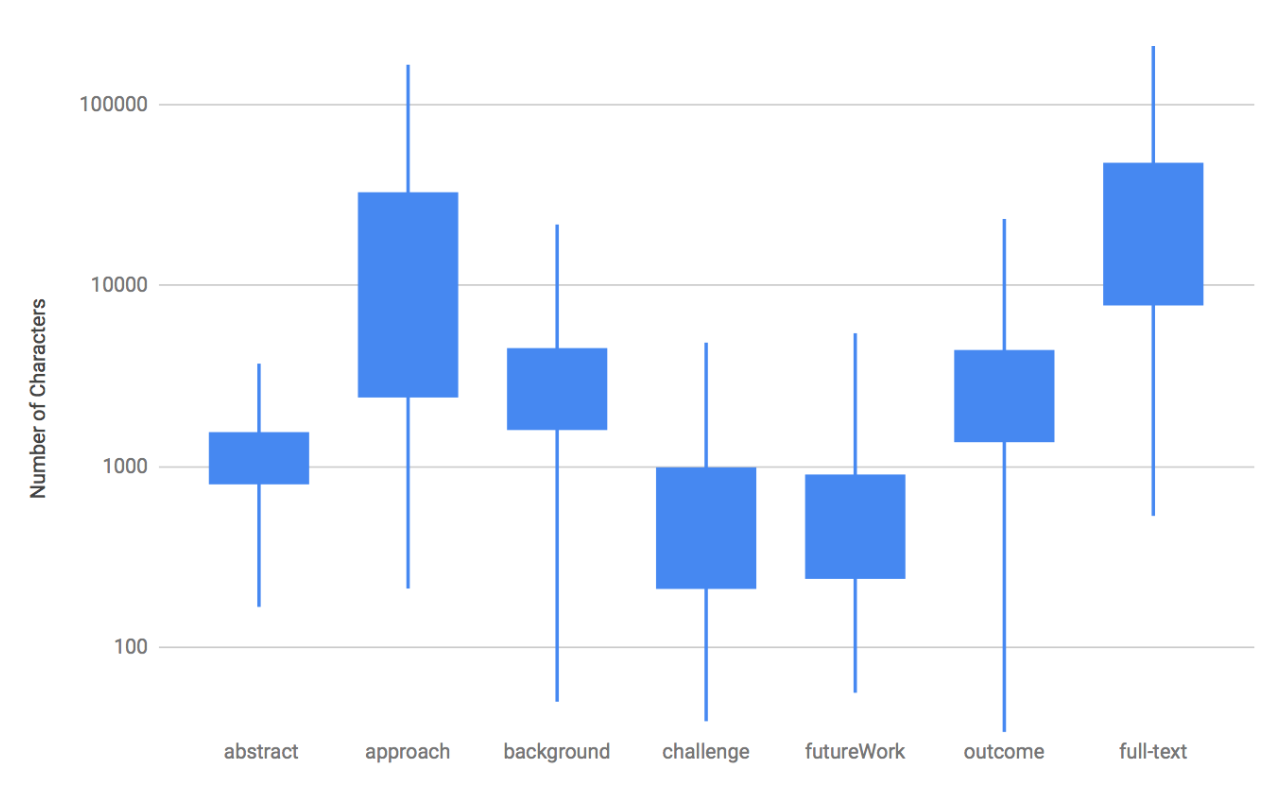
\includegraphics[scale=0.4]{size.png}
  \caption{length of summaries.}
  \label{fig:size}
\end{figure}

\begin{figure}[!htbp]
  \center
  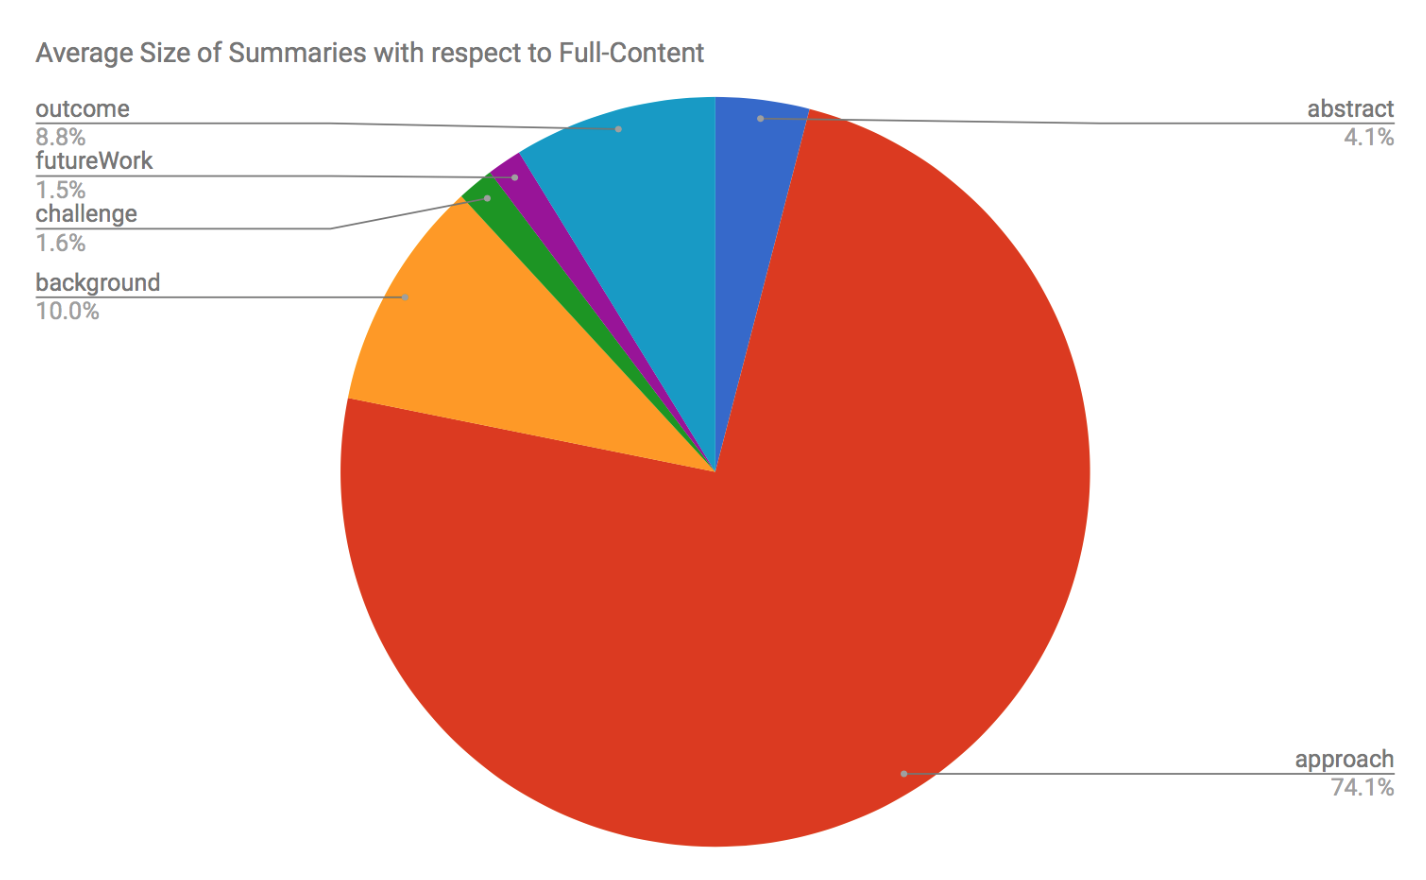
\includegraphics[scale=0.4]{relativeSize.png}
  \caption{length of text parts.}
  \label{fig:relativeSize}
\end{figure}

Since LDA considers documents as \textit{bag-of-words}, the text length (e.g. full-content or summaries) affects the accuracy of the topic distributions inferred by the topic model described in Section~\ref{sec:topicmodel}. The occurrences of words in short texts are less discriminative than in long texts where the model has more word counts to know how words are related \citep{Hong2010}. In view of the above, the \textit{approach}, the \textit{background} and the \textit{outcome} content of a paper generate more accurate topic distributions than those created from other approaches such as the abstract (Figure \ref{fig:size}). Also, the relative presence of each of them in a paper (figure~\ref{fig:relativeSize}) shows an unexpected result when compared to the IMRaD format \citep{Nair2014}. This style proposes to distribute the content of an abstract, and by extension the full-paper, as follows: \textit{Introduction}(25\%), \textit{Methods}(25\%), \textit{Results}(35\%) and \textit{Discussion}(15\%). However, the results (figure~\ref{fig:relativeSize}) show that \textit{Method} section (\textit{approach} content) is more extensive than \textit{Results} section (\textit{outcome} content) in our corpus.

All pairwise similarities between full-papers, abstracts and rhetorical-based summaries are calculated to measure the \textbf{\textit{internal-representativeness}} of a summary with respect to the original text, i.e. the topic-based similarity value (equation~\ref{eq:simcontent}) between the probability distributions of the full-text and each of the summaries. Results (table~\ref{tab:irepresentativeness}) suggest that summaries created from the \textit{approach} content are more representative than others, i.e. the distribution of topics describing the text created from the \textit{approach} content is the most similar to the one corresponding to the full-content of the paper.

\begin{table}[!htb]
    \centering
        \begin{tabular}{l*{6}{c}r}\hline
                        & Min & Lower Quartile & Upper Quartile & Max & Dev  & Median \\
          \hline
          abstract & 0.0489 & 0.9109 & 0.9840 & 1.0000 & 0.1443 & 0.9741 \\
          \textbf{approach} & \textbf{0.0499} & \textbf{0.9969} & \textbf{1.0000} & \textbf{1.0000} & \textbf{0.0872} & \textbf{0.9998} \\
          background & 0.0463 & 0.8967 & 0.9937 & 0.9988 & 0.2037 & 0.9822 \\
          challenge & 0.0426 & 0.7503 & 0.9517 & 0.9940 & 0.2224 & 0.8829 \\
          futureWork & 0.0000 & 0.6003 & 0.9435 & 0.9948 & 0.2842 & 0.8814 \\
          outcome & 0.0485 & 0.9267 & 0.9925 & 0.9990 & 0.1721 & 0.9835 \\
        \end{tabular}
    \caption{ Accuracy results when comparing the most related articles using a summary (e.g. abstract, approach, background, challenge, future work or outcome), with those obtained using the full-text of the article (\textit{internal-representativeness}).}\label{tab:irepresentativeness}
\end{table}

\subsubsection{External-Representativeness}  

The \textit{external-representativeness} metric tries to measure how different is the set of related documents obtained from summaries with respect to those derived from the original full-text. In terms of \textit{precision}, \textit{recall} and \textit{f-measure}, a comparison has been performed to analyze the behavior of the summaries when trying to discover related content compared to use the full-text of the article.

\begin{figure}[!htbp]
  \center
  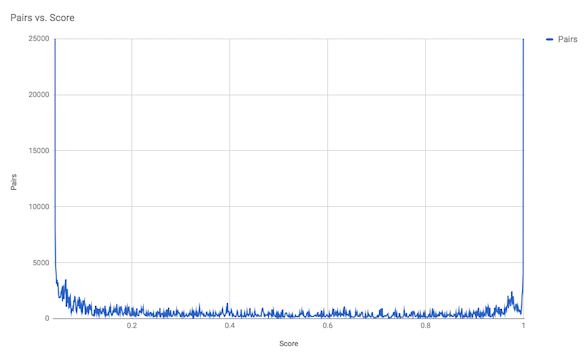
\includegraphics[scale=0.45]{similarities.png}
  \caption{number of pairwises by similarity score (rounded up to two decimals).}
  \label{fig:similarities}
\end{figure}


By using the same topic model previously created, similarities among all pairs of documents were also calculated according to equation~\ref{eq:simcontent}. Then, a minimum score or similarity threshold is required to define when a pair of papers are related. Each threshold is used to create a gold-standard which relates articles to others based on their similarity values. In order to discover that lower bound of similarity, a study about trends in the similarity scores (fig~\ref{fig:similarities}) as well as distributions of topics in the corpus (fig~\ref{fig:articleTopics}) was performed. We can see that topics are not equally balanced across papers. This fact generates separated groups of strongly related papers. We think this phenomena is due to our usage of a corpus created from journals where different domains are equally balanced. Then, we considered a similarity score equals to $0.99$ (fig ~\ref{fig:similarities}) as the threshold from which strong relations appear. However, to cover different interpretations of similarity, from those based on sharing general ideas or themes to those that imply to share a more specific content, the following list of thresholds was considered in the experiments: 0.5, 0.6, 0.7, 0.8, 0.9, 0.95 and 0.99.


For each similarity threshold, a gold-standard was created based on considering as related those papers with a similarity value upper than the selected threshold. Results ( figure ~\ref{fig:precision}) comparing the related papers inferred from the full-content with those inferred from the partial-content representation (i.e. abstract or rhetorical parts) suggest that strongly related papers are mainly discovered by using the summary created from the \textit{approach} section. The reason for this may be based on the average size of this type of summaries or the particular content included in this part of a paper. While other summaries include more general-domain words, the \textit{approach} content includes more specific words that describe the method or the final objective of the paper. So, for higher similarity thresholds, i.e. for strongly related papers, the recommendations discovered by using the \textit{approach} are more precise than those discovered by using the abstract.

\begin{figure}[!htbp]
  \center
  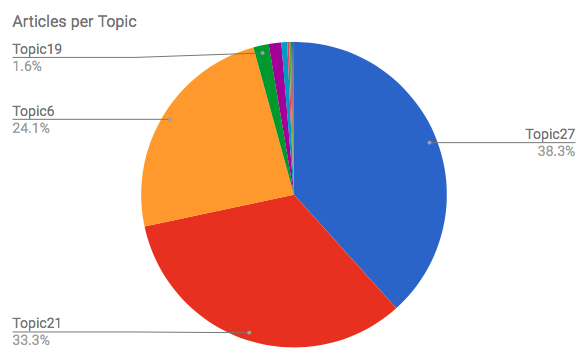
\includegraphics[scale=0.4]{articlesTopic.png}
  \caption{topics per article with value above 0.5.}
  \label{fig:articleTopics}
\end{figure}


In terms of \textit{recall} (figure ~\ref{fig:recall}), the upward trend followed by the \textit{approach}, the \textit{outcome} and the \textit{background} content remarks the assumption of summaries containing key words allow to discover more similar papers than others. Moreover, since \textit{recall} overlooks false-negatives classifications, it suggests that these parts of a research paper share more words than others with strongly related papers but they may also present commonalities with highly related papers, except in case of \textit{approach} which still exhibits higher \textit{precision}.

\begin{figure}[!htbp]
  \center
  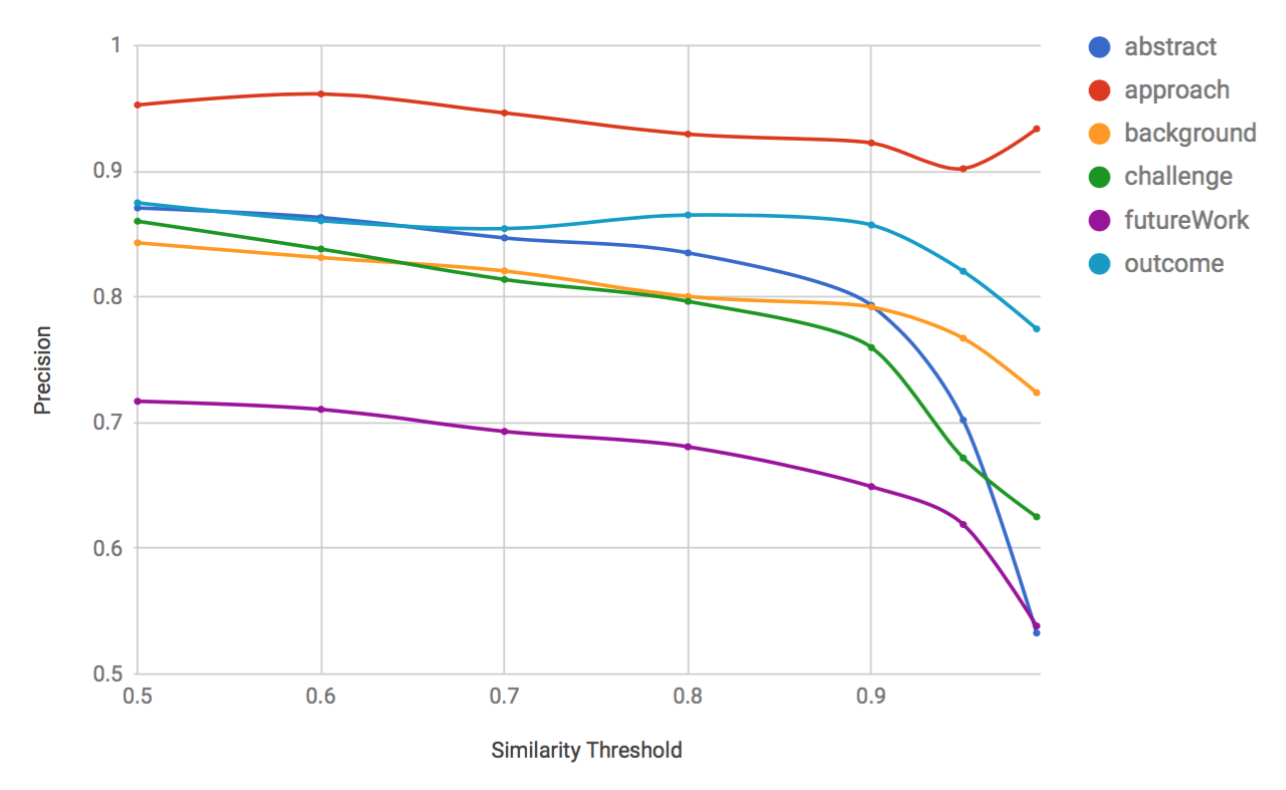
\includegraphics[scale=0.4]{precision.png}
  \caption{Precision at different similarity thresholds.}
  \label{fig:precision}
\end{figure}

\begin{figure}[!htbp]
  \center
  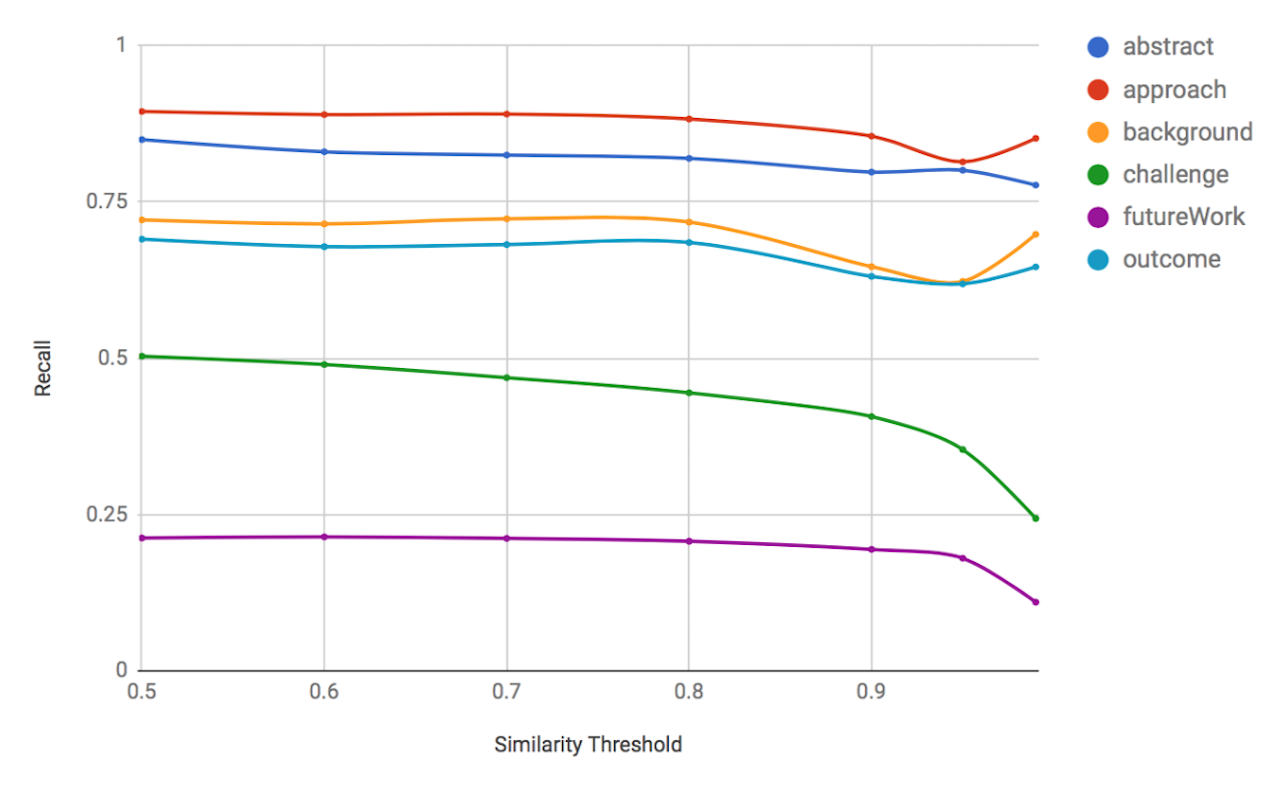
\includegraphics[scale=0.4]{recall.png}
  \caption{Recall at different similarity thresholds.}
  \label{fig:recall}
\end{figure}


As expected, only summaries created from the \textit{approach}, the \textit{outcome} and the \textit{background} content maintain high accuracy values (fig~\ref{fig:fmeasure}) even for high similarity thresholds. Along with the results showed in figure~\ref{fig:stdeviation}, where the same three rhetorical classes present the lowest standard deviation over the \textit{f-measure}, they can be considered as the most robust summaries containing the ideas that better characterize the paper compared to others.


\subsection{Conclusion}
Topic-based relations have been studied among scientific documents based on their abstract sections with respect to summaries corresponding to their scientific discourse categories. For this purpose, two novel measures have been proposed: (1) \textit{internal-representativeness} and (2) \textit{external-representativeness}.

Results show that summaries created from the \textit{approach}, \textit{outcome} or \textit{background} content of a paper describe more accurately its full-content in terms of overall ideas and related documents than abstracts. Although those summaries are more extensive in number of characters than other with similar \textit{precision} such as the abstract content, they have proven to be particularly helpful  discovering strongly related papers, i.e. papers with a similarity value close to 1.0.

\begin{figure}[!htbp]
  \center
  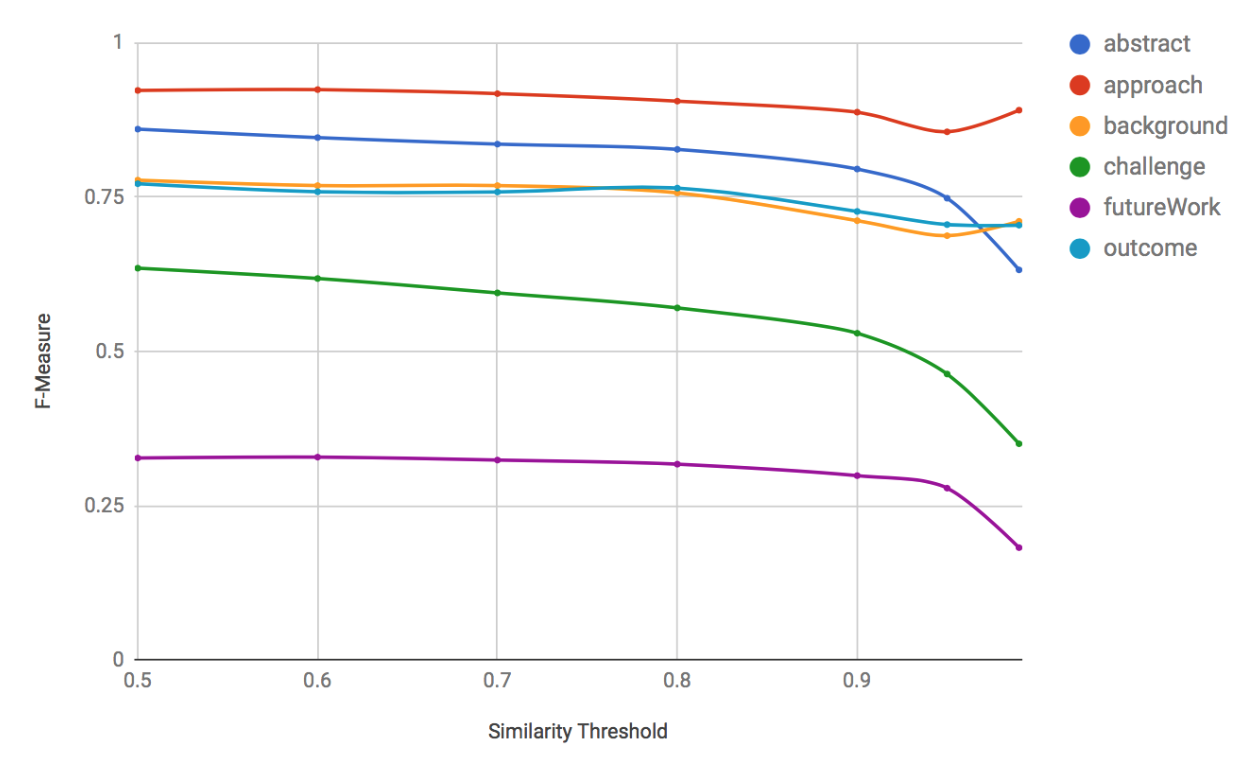
\includegraphics[scale=0.4]{fmeasure.png}
  \caption{f-measure performance.}
  \label{fig:fmeasure}
\end{figure}

\begin{figure}[!htbp]
  \center
  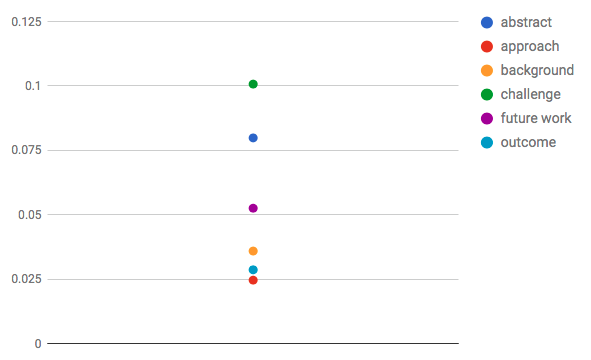
\includegraphics[scale=0.4]{stdeviation.png}
  \caption{f-measure deviation.}
  \label{fig:stdeviation}
\end{figure}


\section{Topic-based Clustering}
\label{sec:topic-clustering}

Once we have a better understanding of the behavior of topic models to represent texts, and the relationships that can be derived from them, we examine their usefulness in browsing document collections. A way to explore the knowledge inside document collections is by moving from one information element to another based on certain criteria that relates them. This approach requires to calculate a similarity matrix with all possible comparisons between elements, so we can later select the most pertinent ones. Since computing a $n \times n$ matrix takes $O(n^2)$ time, obtaining all possible pairs of similarities in a large collection of documents can be unfeasible because of the quadratic cost of comparing every pair of elements.

In order to reduce the complexity, some approaches have introduced mechanisms (mainly pre-election methods) to alleviate the problem of making this calculation over the whole set of pairs in the collection. However those methods are still quite costly.

In this section we propose a novel clustering technique based on topic model distributions that reduces the complexity to find relations between documents in a large corpus of textual documents, without compromising efficiency and providing additional information about relations. A detailed description of our algorithm is given in Section ~\ref{sec:clustering-approach}. The experiments to verify the efficiency and effectiveness of our clustering algorithms using real data, and demonstrate that our approach is competitive enough against both a centroid-based and a density-based clustering baselines are described in Section ~\ref{sec:clustering-experiments}. The most relevant results and conclusions are finally presented in Section ~\ref{sec:clustering-conclusion}.

\begin{figure}
  \centering
  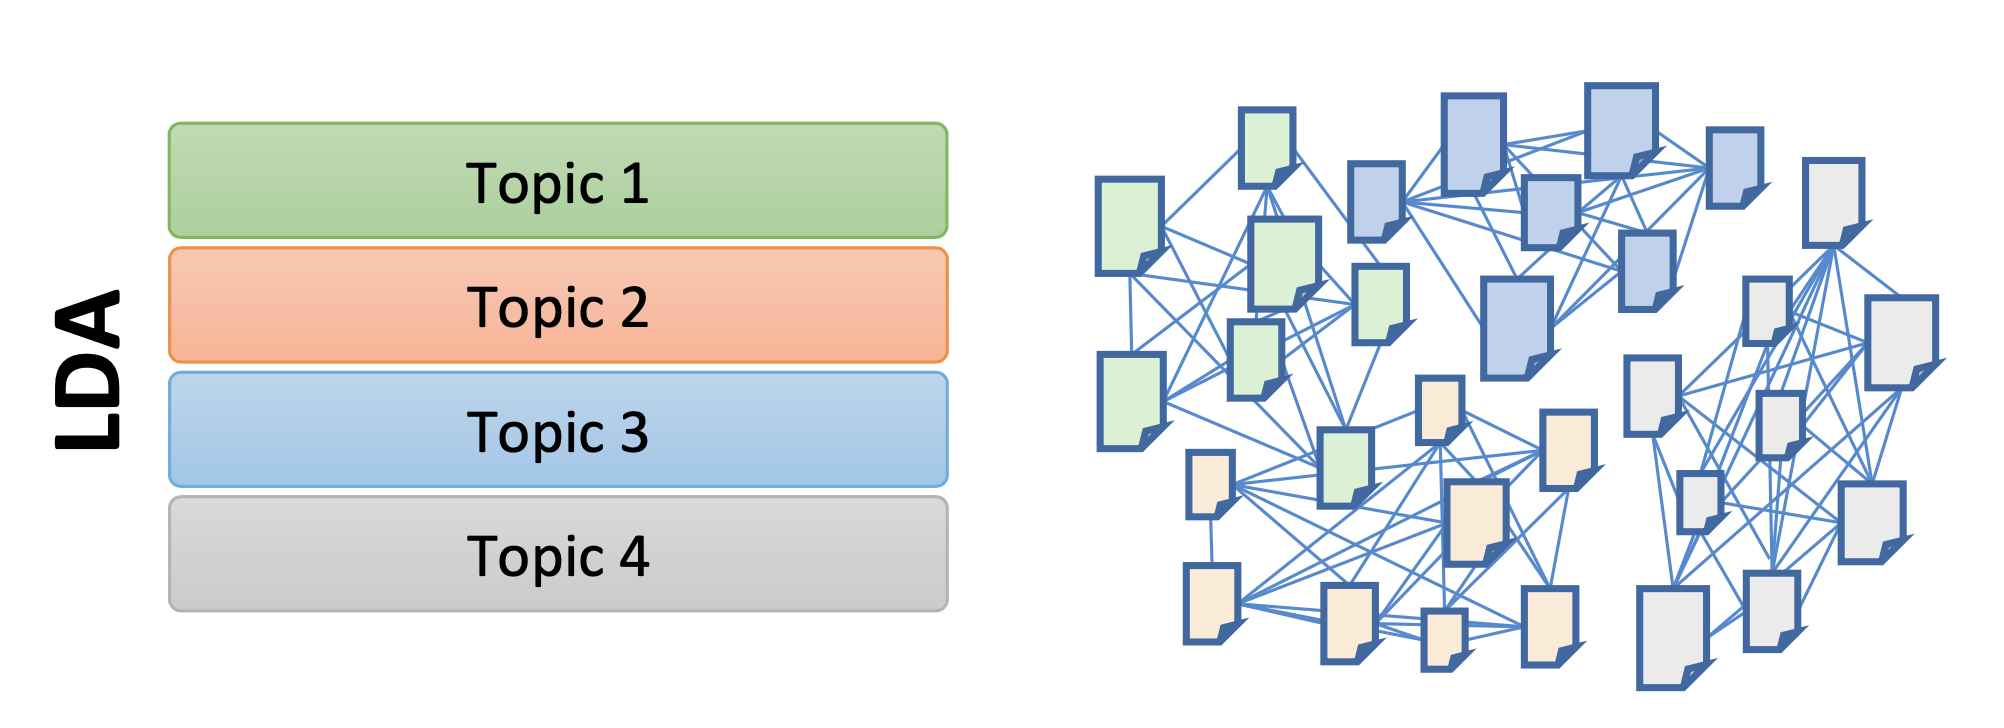
\includegraphics[scale=0.37]{lda-cluster.png}
  \caption{Probabilistic Topic Models, and in particular Latent Dirichlet Allocation (LDA), can efficiently divide the search space and speed up the process of finding relations among documents inside big collections.}
  \label{fig:lda-cluster}
\end{figure}



\subsection{Most Relevant Topics}
\label{sec:clustering-approach}

Our algorithm to identify the most relevant topics draw inspiration from other clustering techniques to divide the initial space of elements into smaller sub-groups where the complexity of calculating all possible distances is significantly reduced. Existing unsupervised approaches based on centroids or density measures require to make comparisons between elements to find groups of similar elements in the collection. They usually follow an iterative methodology to produce the final solution, based on calculating distances between the elements inside each intermediate state. A na{\"i}ve approach would need to calculate all possible distances between elements, which takes $O(n^2)$ time for a $n \times n$ matrix. That makes it impossible to apply such techniques on large collections of documents, since the cost of comparing each element with the others escalates quickly. For those big volumes of data, a clustering task that only takes linear time to discover the clusters can significantly alleviate this problem. For example, a classification method that does not require any other data except the element information to assign the item to the corresponding cluster will take $O(n)$ time to compose those groups.

The classification method needs to take advantage of both the vectorial representations of the documents and the similarity measure used to relate them in a corpus. Since the representational model considered is based on Probabilistic Topic Models (and more specifically on LDA), the classification method leverages on the particular behavior of Dirichlet distributions, which describes each document by a density vector where the sum of all the probability values must be equal to 1.0. Thus, analyzing the relations between the topics that compose a topic distribution becomes more important than comparing their probability values with another topic distribution.

Our hypothesis is that, \textit{given a collection of topic distributions, an unsupervised classification with high precision and linear computing time can be performed by considering only the topic distribution of each document and without needing to further compare it with other document's distributions}.
% \citep{Towne2016}

All algorithms have been compared in terms of \textit{cost}, \textit{effectiveness} and \textit{efficiency} \citep{Halkidi2001a}. \textit{Cost} is based on the number of pairwise similarity checks. \textit{Effectiveness} handles relevance measures such as \textit{precision} and \textit{recall}. And \textit{efficiency} tries to measure the overall balance between \textit{cost} and \textit{effectiveness}. More details about those measures will be included in Section~\ref{sec:clustering-experiments}.

\subsubsection{Trends-based Clustering Method}

Topic distributions are formalized as probability distributions following a Dirichlet distribution, so their probability values sum to 1. In this way, the relevance of a topic is influenced and at the same time influences the relevance of the others items in the distribution. Our first approach named \textit{Trends on Dirichlet distribution-based Clustering} (TDC) considers changes in the relevance, i.e. probability values of the topics instead of directly relying on the scores associated to a given topic distribution (Figure \ref{fig:tdc-cluster}). It expresses the oscillations between topic weights considering a fixed order between them. The order can be any, as long as it remains constant in all distributions. Thus, a \textit{probability-vector} composed by $n$ density values is translated to a \textit{trend-expression} made out of $n-1$ trend-values such as (1) upward, (2) downward and (0) sustained. This \textit{trend-expression} will identify the cluster  the distribution falls into, and therefore the corresponding item belongs to. TDC is defined as:
\begin{equation}
TDC(P)=T
\end{equation}
\begin{conditions}
 T_{i}     & 1,  when $P_i < P_{i+1}$ \\
 T_{i}     & 2,  when $P_i > P_{i+1}$ \\   
 T_{i} 	   & 0,  when $P_i = P_{i+1}$
\end{conditions}
For example, given the distribution $P_1=[0.23, 0.18, 0.33, 0.13, 0.13]$, the assigned cluster will be $T=2120$. The first value is $2$ because $0.23$ is greater than $0.18$ (same for other values).

\begin{figure}[!htbp]
  \centering
  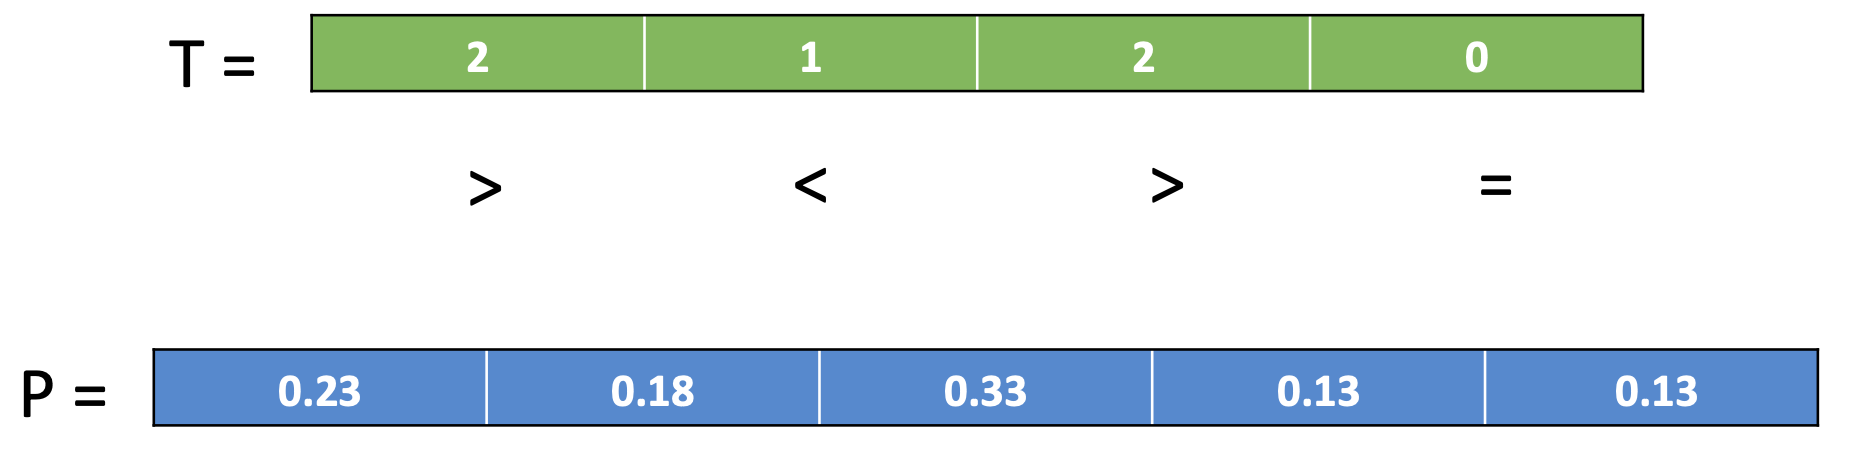
\includegraphics[scale=0.33]{tdc-cluster.png}
  \caption{TDC considers variations across consecutive topics inside a document’s topic distribution.}
  \label{fig:tdc-cluster}
\end{figure}


\subsubsection{Ranking-based Clustering Method}

We propose a clustering technique named \textit{Ranking on Dirichlet distribution-based Clustering} (RDC) that only considers the top $n$ topics from the ranked list of probability distributions to classify similar topic distributions (Figure \ref{fig:rdc-cluster}). It is based on the focal document selection proposed by \citep{Towne2016} to validate LDA-based similarity algorithms against human perception of similarity. RDC is defined as:
\begin{equation}
RDC(P)=R
\end{equation}
where  $\forall i \in R, R_i>=R_{i+1}$ and $\forall j \in P, R_1>=P_j$

This is based on the assumption that the highest weighted topics have a high influence in the rest of topics in terms of calculating distances, when comparing continuous multivariate probability distributions. Since similarity measures (Section ~\ref{sec:related-work}) based on probability distributions are oriented to determine the uncertainty of the distribution, when a mixture of probability distributions is considered, as in the case of Topic Models, the top $n$ distributions (i.e. the most relevant topics) should be sufficient to allow us grouping similar distributions. Taking into account the above considerations, the RDC algorithm classifies a topic distribution according to only $n$ highest probability values. For instance, given the following topic distribution: $P_2=[0.23, 0.18, 0.33, 0.13, 0.13]$, the assigned cluster is \textit{3} from RDC-1 because that is the topic with the highest weight.

\begin{figure}[!htbp]
  \centering
  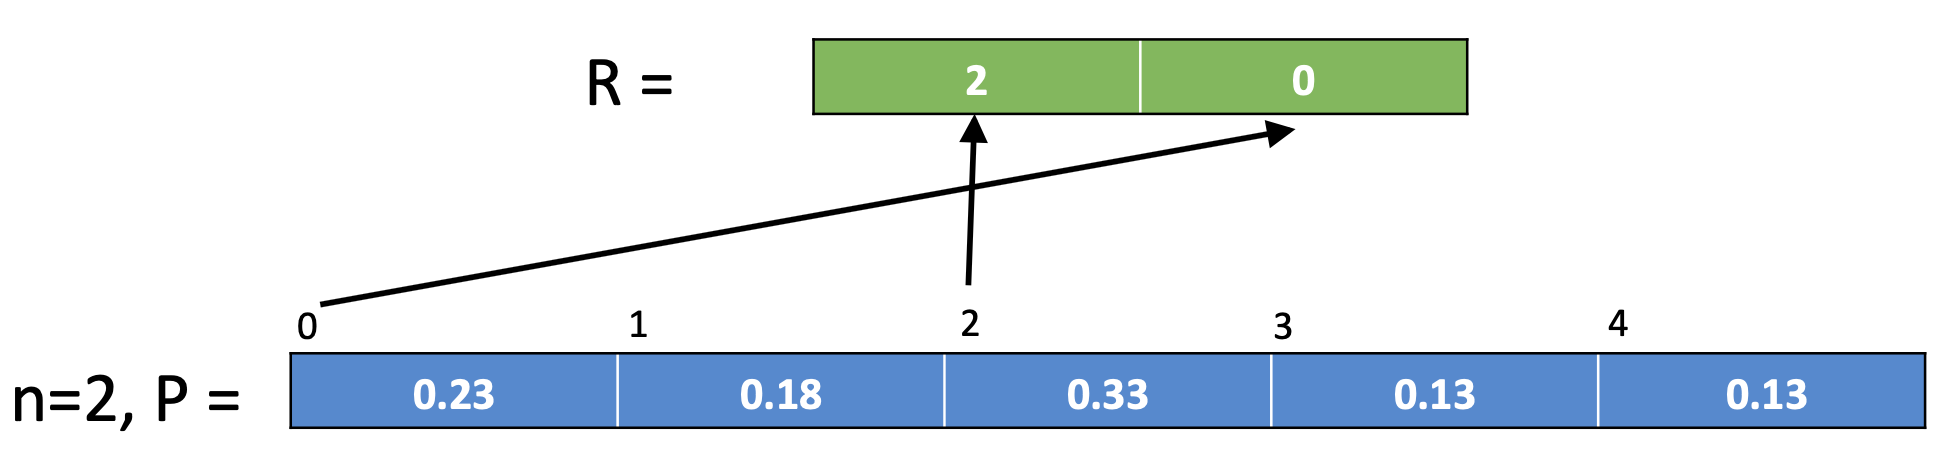
\includegraphics[scale=0.33]{rdc-cluster.png}
  \caption{RDC only considers the top n topics from the ranked list of probability distributions.}
  \label{fig:rdc-cluster}
\end{figure}


\subsubsection{Cumulative Ranking-based Clustering Method}

A variant of the previous algorithm, named \textit{Cumulative Ranking on Dirichlet distribution-based Clustering} (CRDC), also aims to discover the most representative topics that can help to group similar topic distributions. While RDC is based on a fixed number of topics, CRDC is based on the cumulative sum of the weights of the highest topics (Figure \ref{fig:crdc-cluster}). The number of topics is now dynamically determined by a threshold, and once this threshold is reached no more topics are considered. CRDC is defined as:
\begin{equation}
CRDC(P)=C
\end{equation}
where  $\forall i \in C, C_i >=C_{i+1}$ and $\sum\limits_{i=1}^T C_i >= w$ with $T$ size of $C$, and $w$ a cumulative weight threshold.


For instance, considering a CRDC algorithm with a cumulative weight threshold of 0.9, and the following topic distribution: $P_3=[0.36, 0.58, 0.05, 0.01]$. The assigned cluster will be \textit{21}. To come up with this cluster, a ranked list of topics based on their weights is first calculated, $R_p=2|1|3|4$. Then, a sum of weights according to the order described by $R_p$ is performed. When the accumulated sum is greater than the threshold, the topics taking part of the sum will be selected to ``label'' the cluster. In this case, the cumulative weight threshold is 0.9 therefore using only the first two topics we exceed the threshold: $w=0.58+0.36=0.94$

\begin{figure}[!htbp]
  \centering
  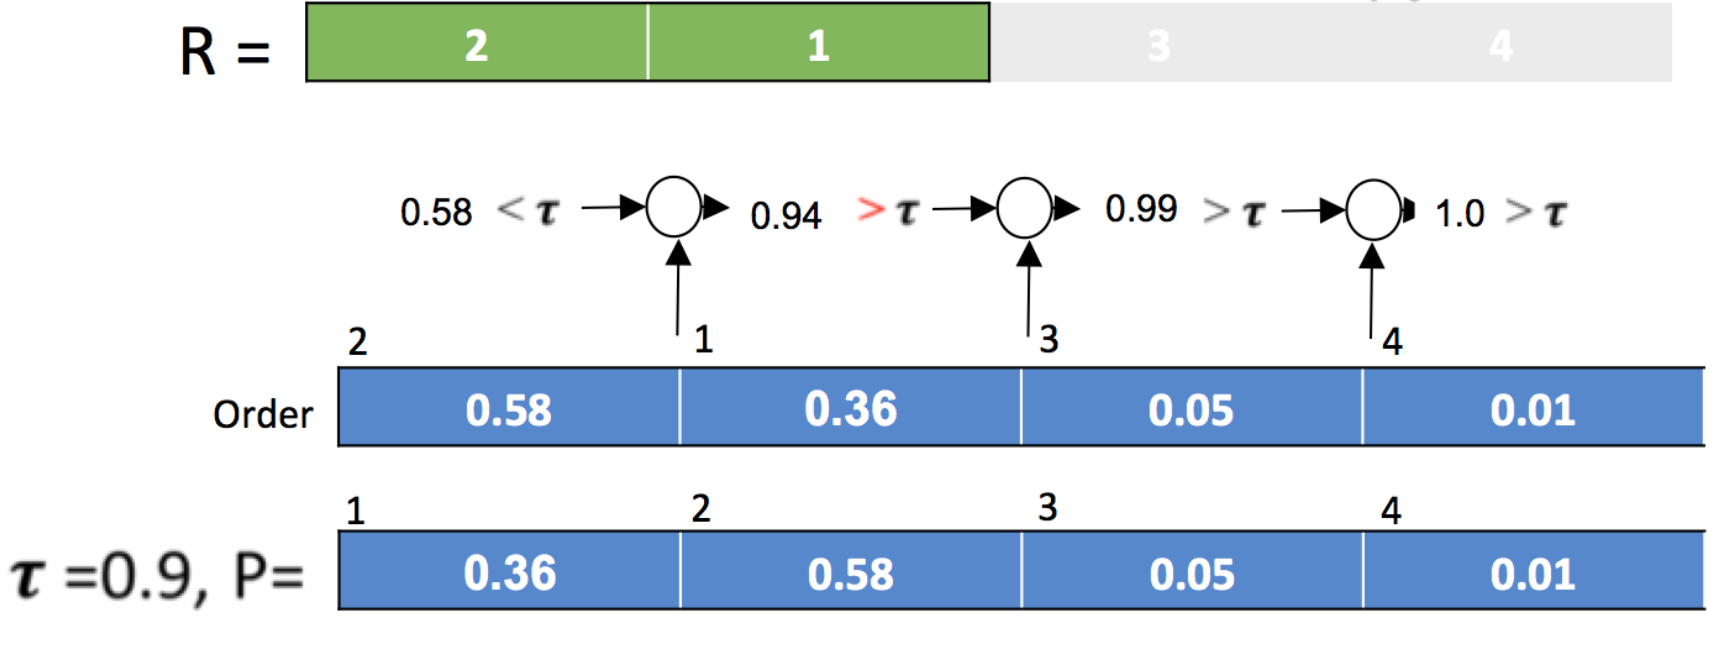
\includegraphics[scale=0.33]{crdc-cluster.png}
  \caption{CRDC only considers the top n topics until the sum of the weights of the highest topics exceeded a given threshold.}
  \label{fig:crdc-cluster}
\end{figure}


\subsection{Evaluation}
\label{sec:clustering-experiments}
In this section we present the experimental setup for evaluating our trends-based (TDC), ranking-based (RDC) and cumulative ranking-based (CRDC) clustering approaches, considering both JS divergence and He distance as similarity measures. We describe the datasets and baseline algorithms that will be used for comparison.

\subsubsection{Datasets}
\label{sec:clustering-datasets}
We used two datasets to evaluate the performance of the algorithms. The first dataset, DIRICHLET-RANDOM-MIXTURE (DRM), is synthetic\footnote{https://doi.org/10.5281/zenodo.931305}. To generate the dataset, we sampled \textit{k} probabilistic distributions from a \textit{randomly k-dimensional selector} based on Dirichlet distributions. This implies that all probabilities must to sum to 1 for each sampled point. The number of sampled points from this mixture of Dirichlet distributions is $n=1000$.

The second dataset has been created from a collection of research papers published in the \textit{Advances in Engineering Software} (AIES) journal. They were retrieved from the Springer API by using the librAIry \citep{Badenes-Olmedo2017} framework and a Topic Model based on LDA was created from them. The sample is also composed by $n=1000$ documents.

Topic models were trained from these datasets by using the criteria described by \citep{Steyvers2006}: $\alpha= 50/k$ , $\beta= 0.01$ and $k=2*(\sqrt{(n/2)})$, where $k$ is the number of topics and $n$ is the number of documents. Since both datasets contain $1000$ documents ($n$), the hyper-parameters $\alpha$ and $\beta$ are assigned as follow: $\alpha=1.136$, and $\beta=0.01$, and the number of topics is fixed to $k=44$. Further tuning of the settings is not crucial in this evaluation process, because we are not focusing on the quality of the model but on the efficiency when calculating similarities from their representational distributions.

\subsubsection{Settings}
\label{sec:clustering-threshold}
Since there is no unified criteria to select a threshold inside the distance scores spectrum that allows us to determine when two documents are similar, we decided to study the distribution of similarity values calculated from all pairwise comparisons. In Figure ~\ref{fig:similarityThreshold}, the result of grouping all similarities by the two most representative decimals, i.e. the first two decimals of the similarity value, is shown. Then, a polynomial function (red line) is approximated to describe the trend of these values. In this function, the similarity score $0.83$ emerges as a global minimum and has been used for filtering out the non-similar document pairs.

\begin{figure}[!htbp]
  \centering
  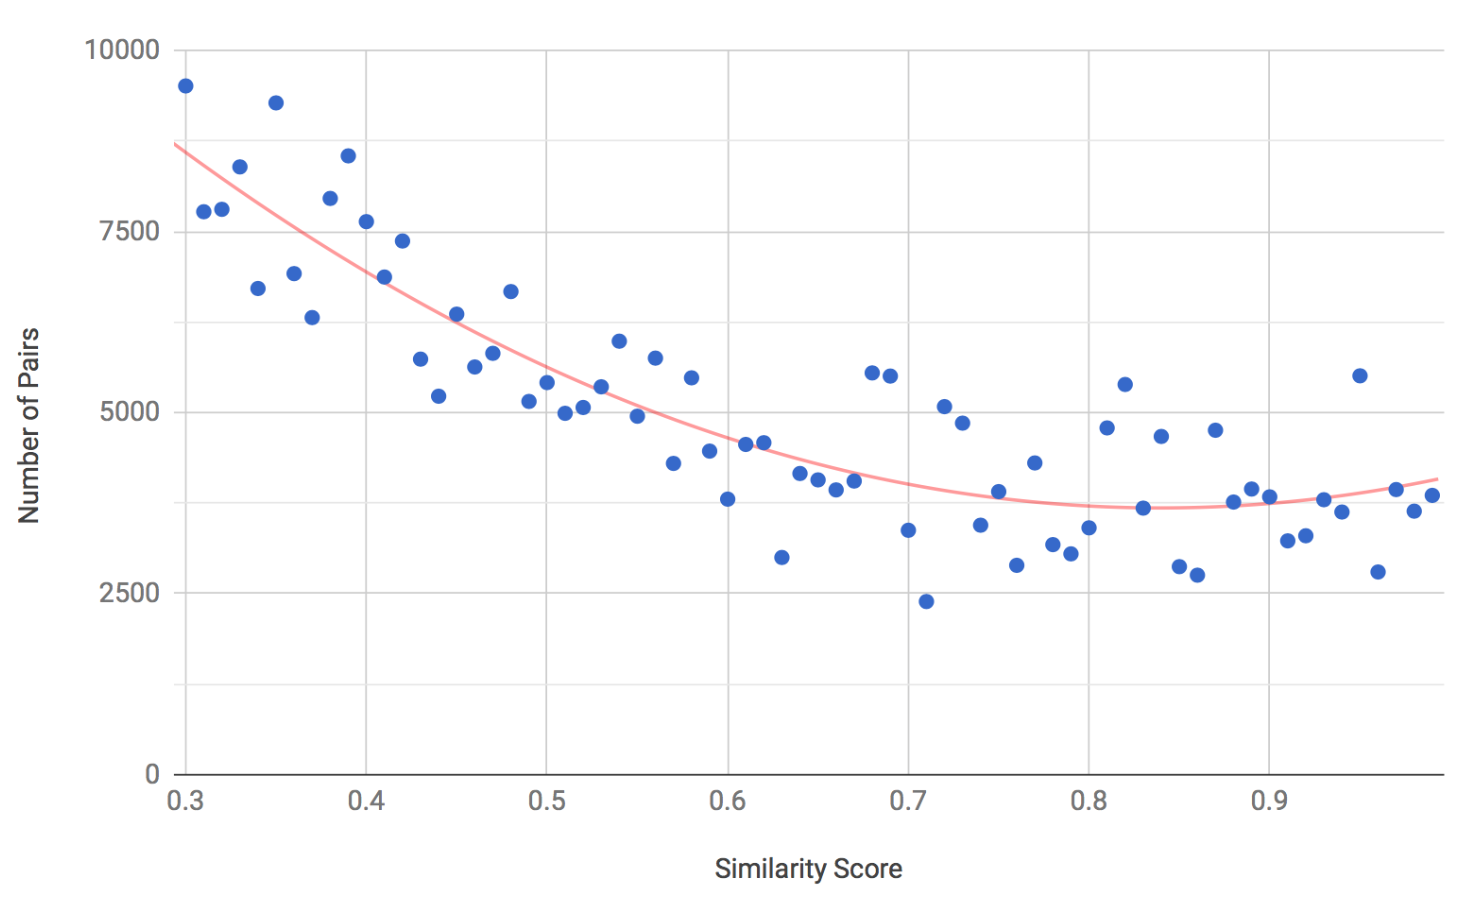
\includegraphics[scale=0.43]{similarity-threshold.png}
  \caption{Similarity values grouped by frequency in AIES}
  \label{fig:similarityThreshold}
\end{figure}

\subsubsection{Baselines}

We compare the performance of TDC, RDC and CRDC algorithms against the following baselines:
\begin{itemize}
  \item \textit{K-Means} as a centroid-based clustering approach.
  \item \textit{DBSCAN} as a density-based clustering approach.
  \item \textit{Random}, which randomly selects $R$ from the dataset
\end{itemize}

Initially, \textit{K-Means} \citep{Bahmani2012} randomly composes a set of centroids and assigns each point of the sample to its nearest cluster based on a distance measure. Then, a new set of centroids is calculated from the previous ones according to the assigned points. This process is repeated until the set of centroids does not change significantly between consecutive iterations or a maximum number of iterations is reached. The \textit{scalable K-Means} approach used in our experiments is an improved version of \textit{k-means} which obtains an initial set of centers ideally close to the optimum solution. The algorithm implemented at the Apache Commons Math library \footnote{ http://commons.apache.org/proper/commons-math/} was used in the experiments. Based on empirical results, the best configuration is: $k=number-of-topics=44$ and $maxIterations=50$

A widely known density-based algorithm is \textit{DBSCAN} \citep{Ester1996}, which compose clusters from the neighborhood of each point considering at least a minimum number of points and a given radius. Thus, it requires to specify the radius of the point's neighborhood, \textit{Eps}, and the minimum number of points in the neighborhood \textit{MinPts}. Based on empirical results, the best results were obtained with the following configuration: $eps=0.1$ and $minPts=50$

The \textit{Random} algorithm takes as input a parameter \textit{m} and randomly divides the dataset into \textit{m} equal-sized groups of similar documents. For the evaluation, $m$ was set to the number of topics, the dimension of the dataset.

With respect to the proposed algorithms and taking into account empirical results, the RDC algorithm is set to use the \textit{top1} highest topics, and the cumulative weight threshold for the CRDC algorithm is set to $0.9$.

\subsubsection{Measures}

A gold-standard is created for each dataset and distance metric considered. They are created by calculating all pairwise similarities from their documents. Since the $n \times n$ similarity matrix requires $O(n^2)$ time to be calculated, the selected size of datasets has not been too large $n=1000$.

We considered three measures to evaluate our algorithms with respect to the baseline:
\begin{itemize}
  \item \textbf{\textit{cost}}: based on the number of similarity score calculations required by the algorithm:
\begin{equation}
cost=(reqSim - minSim)/(totalSim - minSim)
\end{equation}
The \textit{minSim} corresponds to the number of similar documents obtained from using the \textit{threshold} score previously mentioned in section ~\ref{sec:clustering-threshold}. The \textit{totalSim} corresponds to the Cartesian product of existing documents: $totalSim=n*n=1,000,000$. And the \textit{reqSim} corresponds to the number of similarities calculated by the algorithm.
  \item \textbf{\textit{effectiveness}}: based on $precision$ and $recall$. It expresses the quality of the algorithm:
\begin{equation}
 effectiveness = \frac{precision^2  + recall^2}{2}
\end{equation}
  \item \textbf{\textit{efficiency}}: based on the previous ones, it express a compromise between quality and performance:
\begin{equation}
 efficiency = effectiveness - cost
\end{equation}
\end{itemize}

\subsubsection{Results}
\label{sec:clustering-results}

The source code used to evaluate the algorithms along with the results obtained are publicy available\footnote{https://doi.org/10.5281/zenodo.931305}.

In terms of \textbf{\textit{effectiveness}} (Figures ~\ref{fig:effectivenessJS} and ~\ref{fig:effectivenessHe}), the results highlight that \textit{K-Means} and \textit{CRDC} outperform the other algorithms. \textit{K-Means} was expected to be a top performer because the algorithm itself performs comparisons to map clusters. The fact that \textit{CRDC} has such good performance encourages us to think that, in fact, the most relevant topics when they altogether exceed a certain high weight threshold, are those that best represent the document and allow to group together similar documents. However, as shown in tables ~\ref{tab:precisionJS}, ~\ref{tab:precisionHe}, ~\ref{tab:recallJS} and ~\ref{tab:recallHe}, considering a fixed number of more relevant topics (\textit{RDC}) or considering the trend of their weights (\textit{TDC}) does not seem to perform so well on aggregating similar documents, since their \textit{precision} and \textit{recall} values are very low in both cases. It is surprising that the \textit{DBSCAN} has such low value. Taking a look at its \textit{precision} and \textit{recall} values, and also seeing the number of groups that each algorithm has created (Figure ~\ref{fig:clusters}), we believe that having a corpus containing a very cohesive set of documents (all papers in corpus belong to the same journal) affects the performance of this algorithm since it divides the corpus into a lower number of groups. This way, it obtains high values of \textit{recall} because most of the pair-wise distances are computed, but very low \textit{precision}.

The results also show that the behavior of the algorithms does not differ significantly when using different similarity measures, for example JS divergence (Figure ~\ref{fig:effectivenessJS}) and He distance (Figure ~\ref{fig:effectivenessHe}). This highlights the importance of the documents' topic distributions to successfully classify them into smaller groups of similar items, while other particular aspects such as the distance or similarity metric used to compare them are less influential.

\begin{figure}[!htb]\centering
  \center
  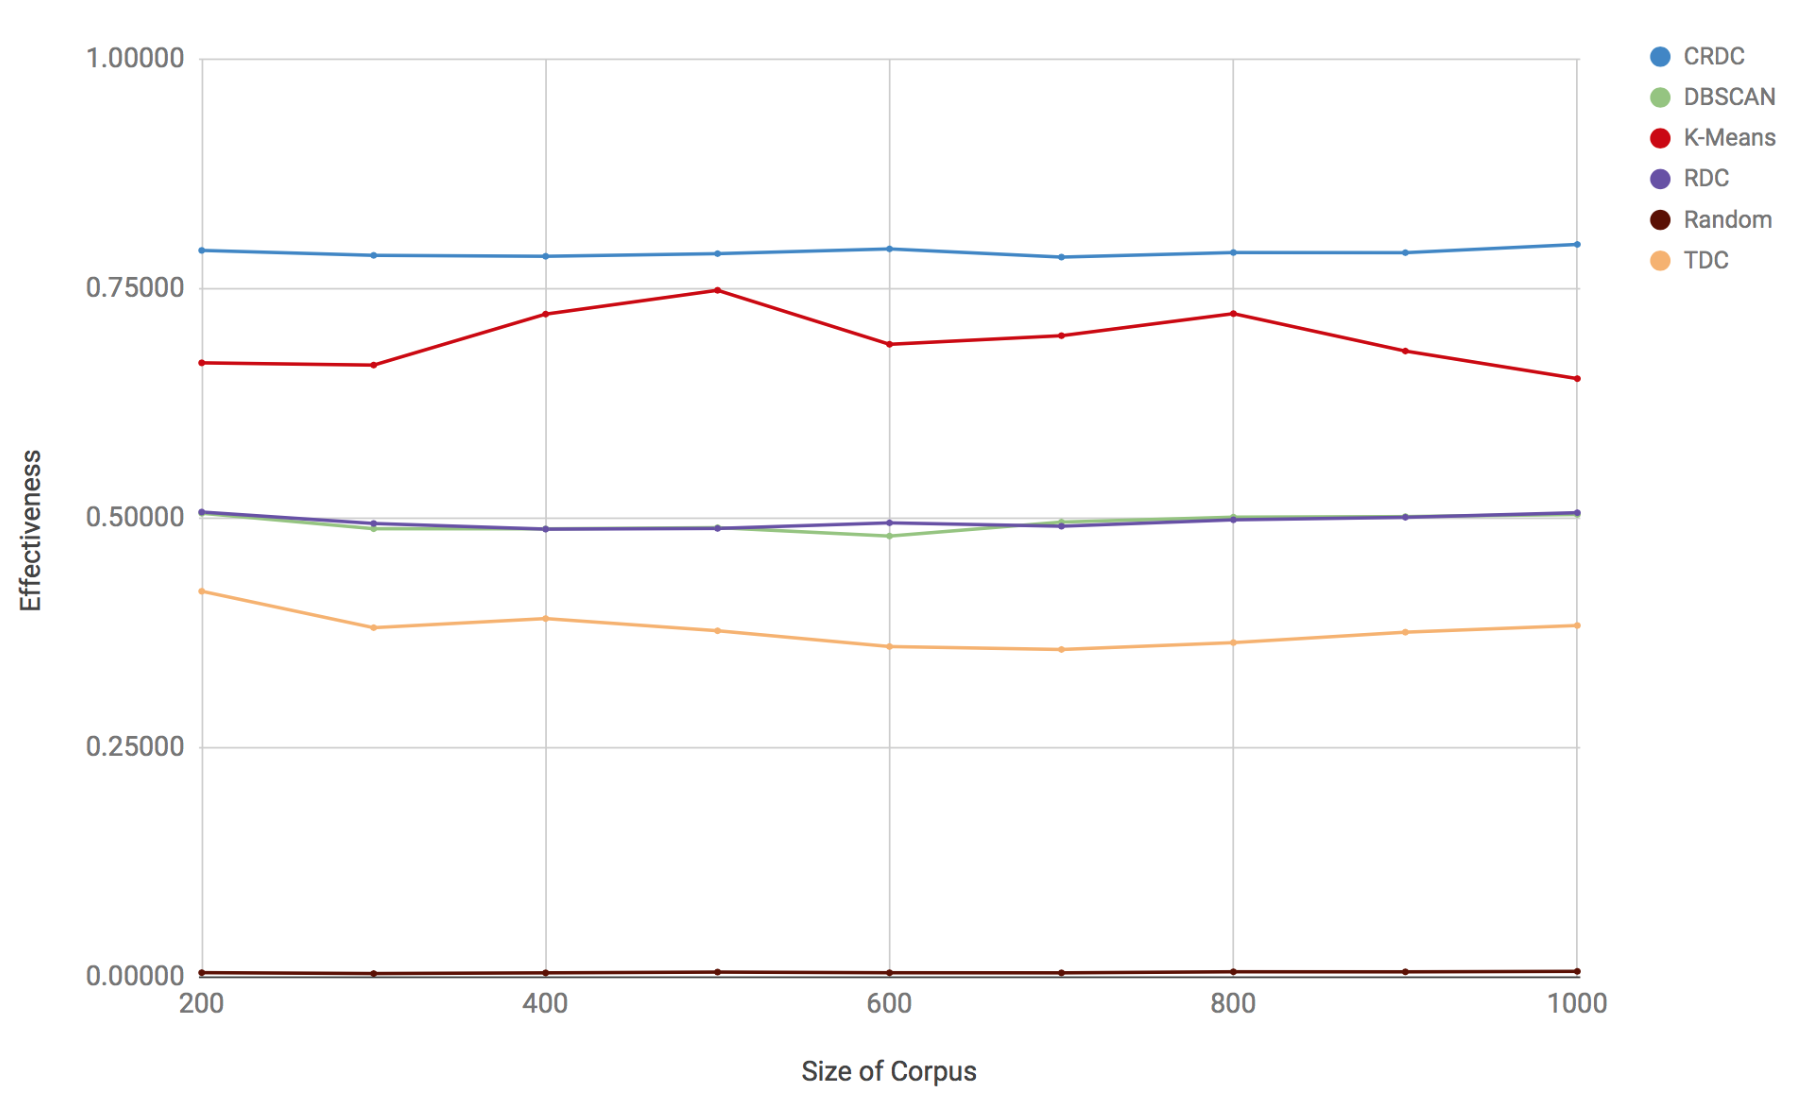
\includegraphics[scale=0.35]{effectivenessJS.png}
  \caption{Effectiveness (JS-based) in AIES}
  \label{fig:effectivenessJS}
\end{figure}

\begin{figure}[!htb]\centering
  \center
  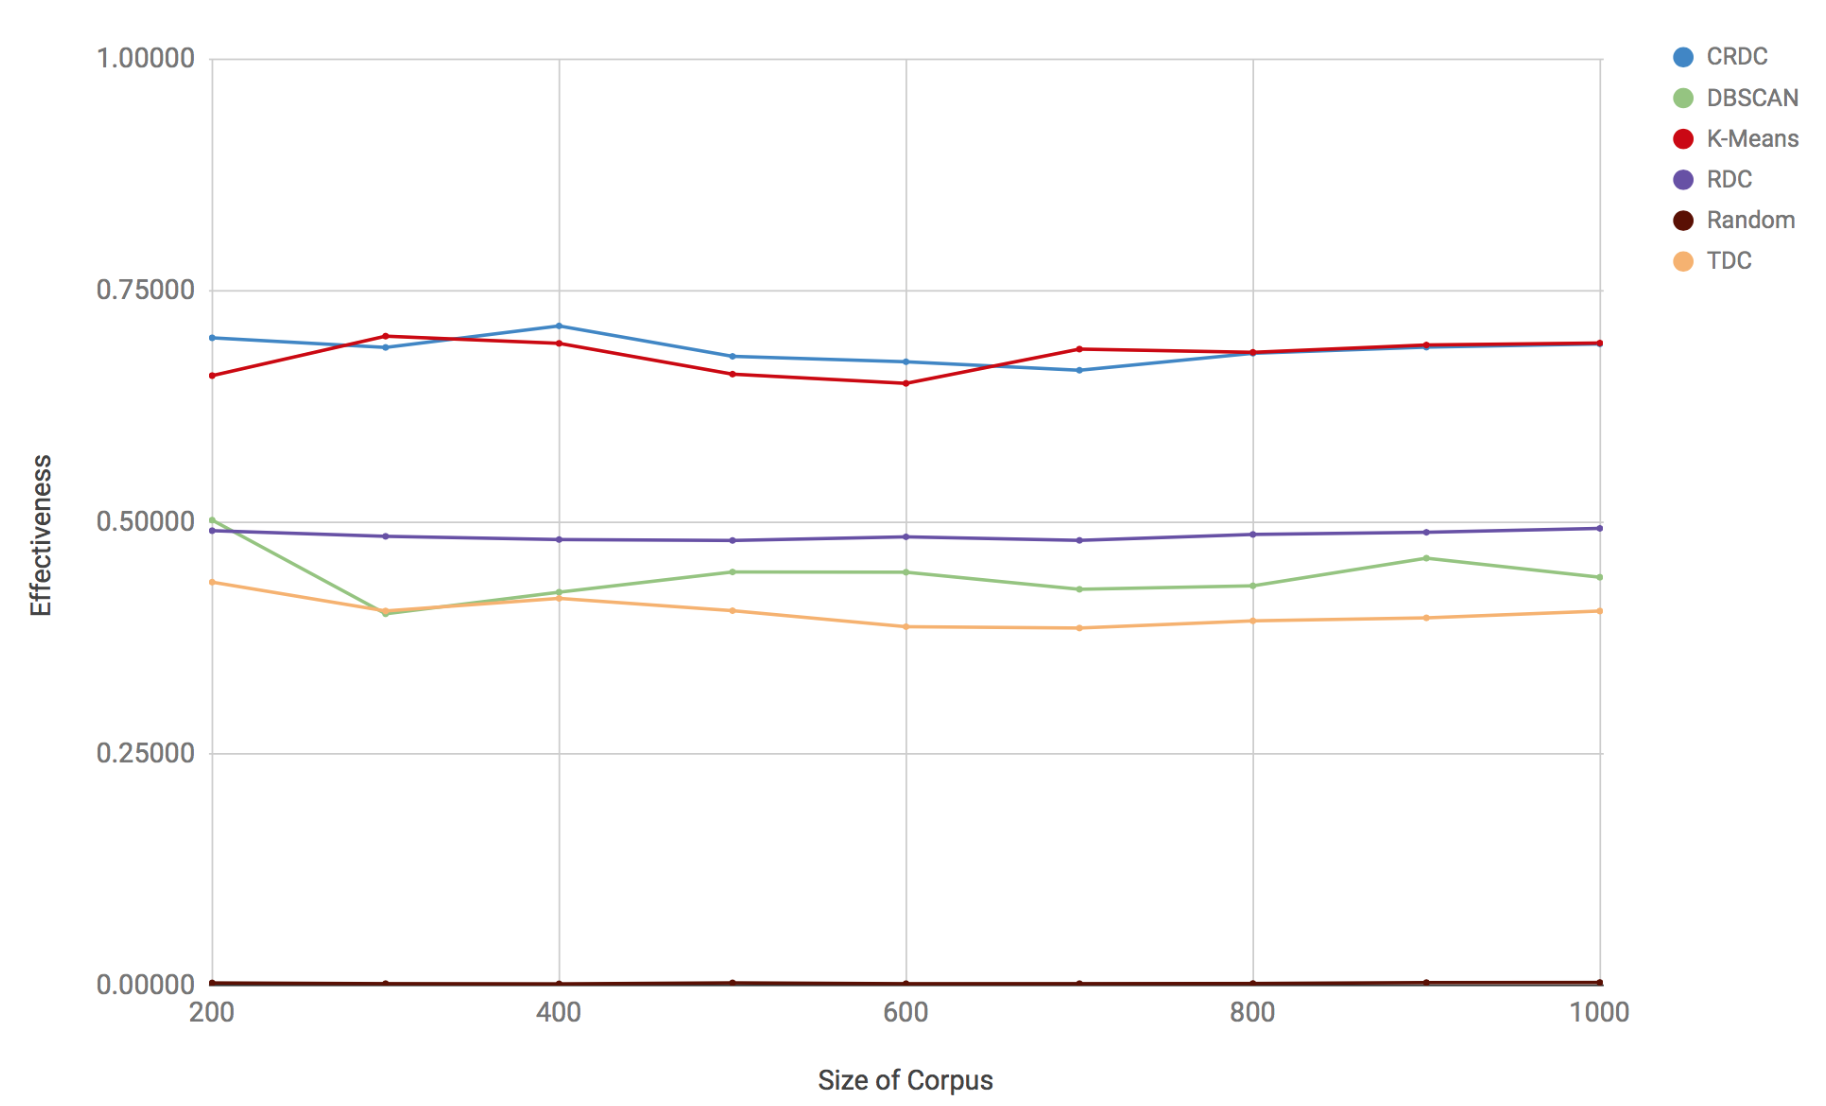
\includegraphics[scale=0.35]{effectivenessHe.png}
  \caption{Effectiveness (He-based) in AIES}
  \label{fig:effectivenessHe}
\end{figure}

\begin{figure}[!htb]\centering
  \center
  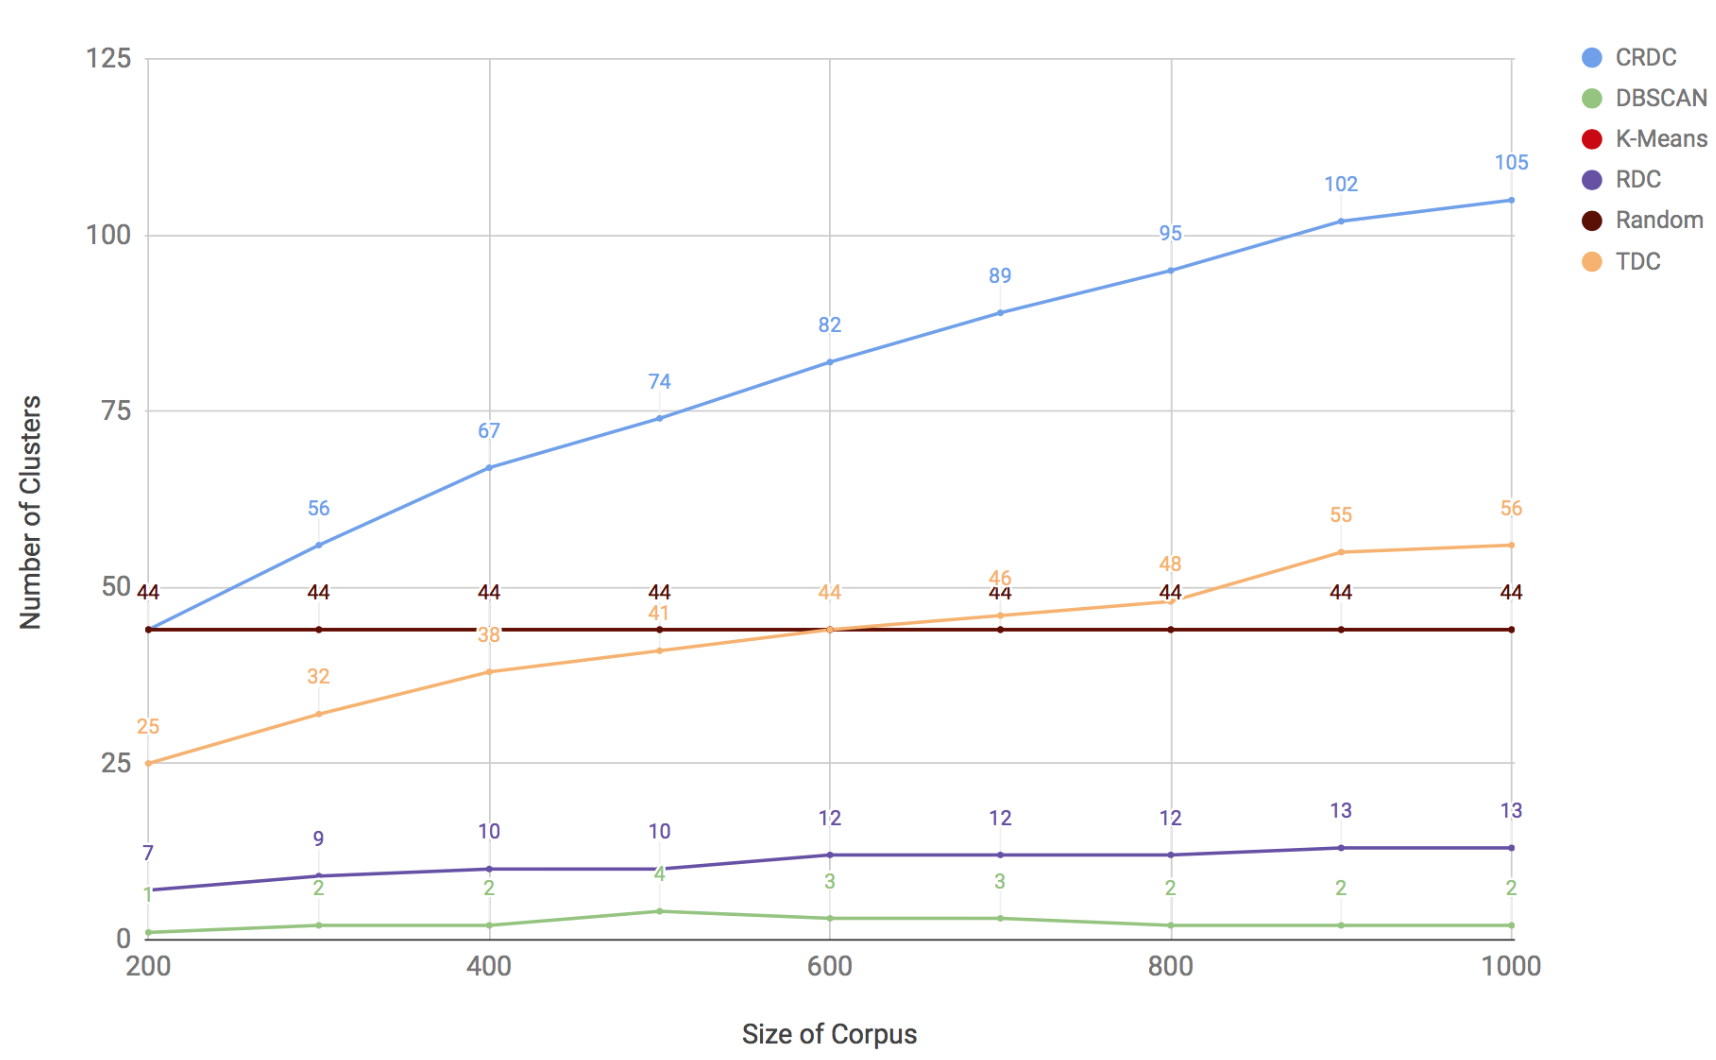
\includegraphics[scale=0.45]{clusters.png}
  \caption{Clusters in AIES}
  \label{fig:clusters}
\end{figure}

% table precision of algorithms
\begin{table}[!htb]
    \centering
        \begin{tabular}{l*{6}{c}r}\hline
                    Size    & CRDC & DBSCAN & K-Means & RDC & TDC  & Random \\
          \hline
					200 & 0.94 & 0.10 & \textbf{0.96} & 0.31 & 0.42 & 0.12 \\
					300 & 0.93 & 0.15 & \textbf{0.94} & 0.30 & 0.39 & 0.08 \\
					400 & \textbf{0.93} & 0.15 & 0.89 & 0.29 & 0.39 & 0.09 \\
					500 & \textbf{0.92} & 0.30 & 0.90 & 0.28 & 0.38 & 0.09 \\
					600 & \textbf{0.92} & 0.19 & 0.88 & 0.28 & 0.38 & 0.08 \\
					700 & \textbf{0.92} & 0.20 & 0.91 & 0.28 & 0.38 & 0.09 \\
					800 & \textbf{0.92} & 0.12 & 0.89 & 0.30 & 0.39 & 0.10 \\
					900 & \textbf{0.92} & 0.13 & 0.87 & 0.30 & 0.40 & 0.10 \\
					1000 & \textbf{0.93} & 0.13 & 0.90 & 0.30 & 0.40 & 0.10 \\
        \end{tabular}
    \caption{Precision (JS-based) in AIES}\label{tab:precisionJS}
\end{table}

\begin{table}[!htb]
    \centering
        \begin{tabular}{l*{6}{c}r}\hline
                    Size  & CRDC & DBSCAN & K-Means & RDC & TDC  & Random \\
          \hline
					200 & 0.75 & 0.07 & \textbf{0.84} & 0.23 & 0.08 & 0.33 \\
					300 & 0.74 & 0.08 & \textbf{0.83} & 0.23 & 0.06 & 0.32 \\
					400 & \textbf{0.76} & \textbf{0.09} & 0.76 & 0.22 & 0.06 & 0.32 \\
					500 & 0.73 & 0.08 & \textbf{0.74} & 0.21 & 0.08 & 0.31 \\
					600 & 0.72 & 0.08 & \textbf{0.73} & 0.21 & 0.06 & 0.30 \\
					700 & 0.71 & 0.10 & \textbf{0.76} & 0.21 & 0.06 & 0.30 \\
					800 & 0.73 & 0.11 & \textbf{0.78} & 0.22 & 0.07 & 0.31 \\
					900 & 0.73 & 0.12 & \textbf{0.80} & 0.22 & 0.08 & 0.32 \\
					1000 & 0.74 & 0.15 & \textbf{0.77} & 0.23 & 0.08 & 0.32 \\
        \end{tabular}
    \caption{Precision (He-based) in AIES}\label{tab:precisionHe}
\end{table}

% table recall of algorithms
\begin{table}[!htb]
    \centering
        \begin{tabular}{l*{6}{c}r}\hline
                    Size  & CRDC & DBSCAN & K-Means & RDC & TDC  & Random \\
          \hline
					200  & 0.92  & \textbf{1.00}  & 0.79  & 0.96  & 0.02  & 0.87 \\
					300  & 0.91  & 0.89  & 0.84  & \textbf{0.96}  & 0.02  & 0.84 \\
					400  & 0.92  & 0.92  & 0.90  & \textbf{0.96}  & 0.02  & 0.86 \\
					500  & 0.91  & 0.94  & 0.88  & \textbf{0.96}  & 0.03  & 0.85 \\
					600  & 0.91  & 0.94  & 0.87  & \textbf{0.96}  & 0.02  & 0.83 \\
					700  & 0.91  & 0.92  & 0.90  & \textbf{0.96}  & 0.02  & 0.83 \\
					800  & 0.92  & 0.92  & 0.88  & \textbf{0.96}  & 0.02  & 0.83 \\
					900  & 0.92  & 0.95  & 0.86  & \textbf{0.96}  & 0.02  & 0.83 \\
					1000  & 0.92  & 0.93  & 0.89  & \textbf{0.97}  & 0.02  & 0.84 \\
        \end{tabular}
    \caption{Recall (JS-based) in AIES}\label{tab:recallHe}
\end{table}

\begin{table}[!htb]
    \centering
        \begin{tabular}{l*{6}{c}r}\hline
                    Size`  & CRDC & DBSCAN & K-Means & RDC & TDC  & Random \\
          \hline
					200 & 0.84 & \textbf{1.00} & 0.65 & 0.96 & 0.02 & 0.82 \\
					300 & 0.84 & \textbf{0.98} & 0.76 & 0.95 & 0.02 & 0.78 \\
					400 & 0.84 & \textbf{0.98} & 0.79 & 0.94 & 0.02 & 0.79 \\
					500 & 0.85 & 0.94 & 0.87 & \textbf{0.95} & 0.02 & 0.78 \\
					600 & 0.86 & \textbf{0.96} & 0.80 & 0.95 & 0.02 & 0.76 \\
					700 & 0.85 & \textbf{0.98} & 0.80 & 0.95 & 0.02 & 0.76 \\
					800 & 0.85 & \textbf{0.99} & 0.81 & 0.95 & 0.02 & 0.76 \\
					900 & 0.85 & \textbf{0.99} & 0.75 & 0.95 & 0.02 & 0.77 \\
					1000 & 0.86 & \textbf{1.00} & 0.74 & 0.96 & 0.02 & 0.78 \\
        \end{tabular}
    \caption{Recall (He-based) in AIES}\label{tab:recallJS}
\end{table}



In terms of \textbf{\textit{cost}} (Figures ~\ref{fig:costJS} and ~\ref{fig:costHe}), the best clustering algorithm, as expected, is based on \textit{random} selection. This is due to the fact that the number of pairs compared by this algorithm is always the minimum, given the dataset is simply randomly divided into \textit{m} equal-sized groups, where \textit{m} is equals to the number of topics, i.e. dimension of the dataset. Since \textit{K-Means} and \textit{DBSCAN} make comparisons between documents until their internal condition is satisfied, they are the most inefficient approaches. \textit{K-Means} involves the highest cost because it compares all the documents with the 44 centroids in each iteration.

Among our proposals, the main reason for an algorithm to present a higher cost is due to the number of groups the corpus is divided into (see Figure ~\ref{fig:clusters}). The greater the number of groups, the fewer the number of later comparisons that have to be made and, therefore, the lower the cost of the algorithm.

The behavior of the \textit{DBSCAN} algorithm depends remarkably on the similarity metric used. We think that this may be due to the way in which both measures satisfy the triangle inequality condition, since one is based on divergence (JS) and the other on distance (He). This property, which defines $distance(a,b) \leq distance(a,c) + distance(c,b)$, is very important in the calculations that \textit{DBSCAN} makes to discover the groups, since it only calculates the distances between near points.

\begin{figure}[!htb]\centering
  \center
  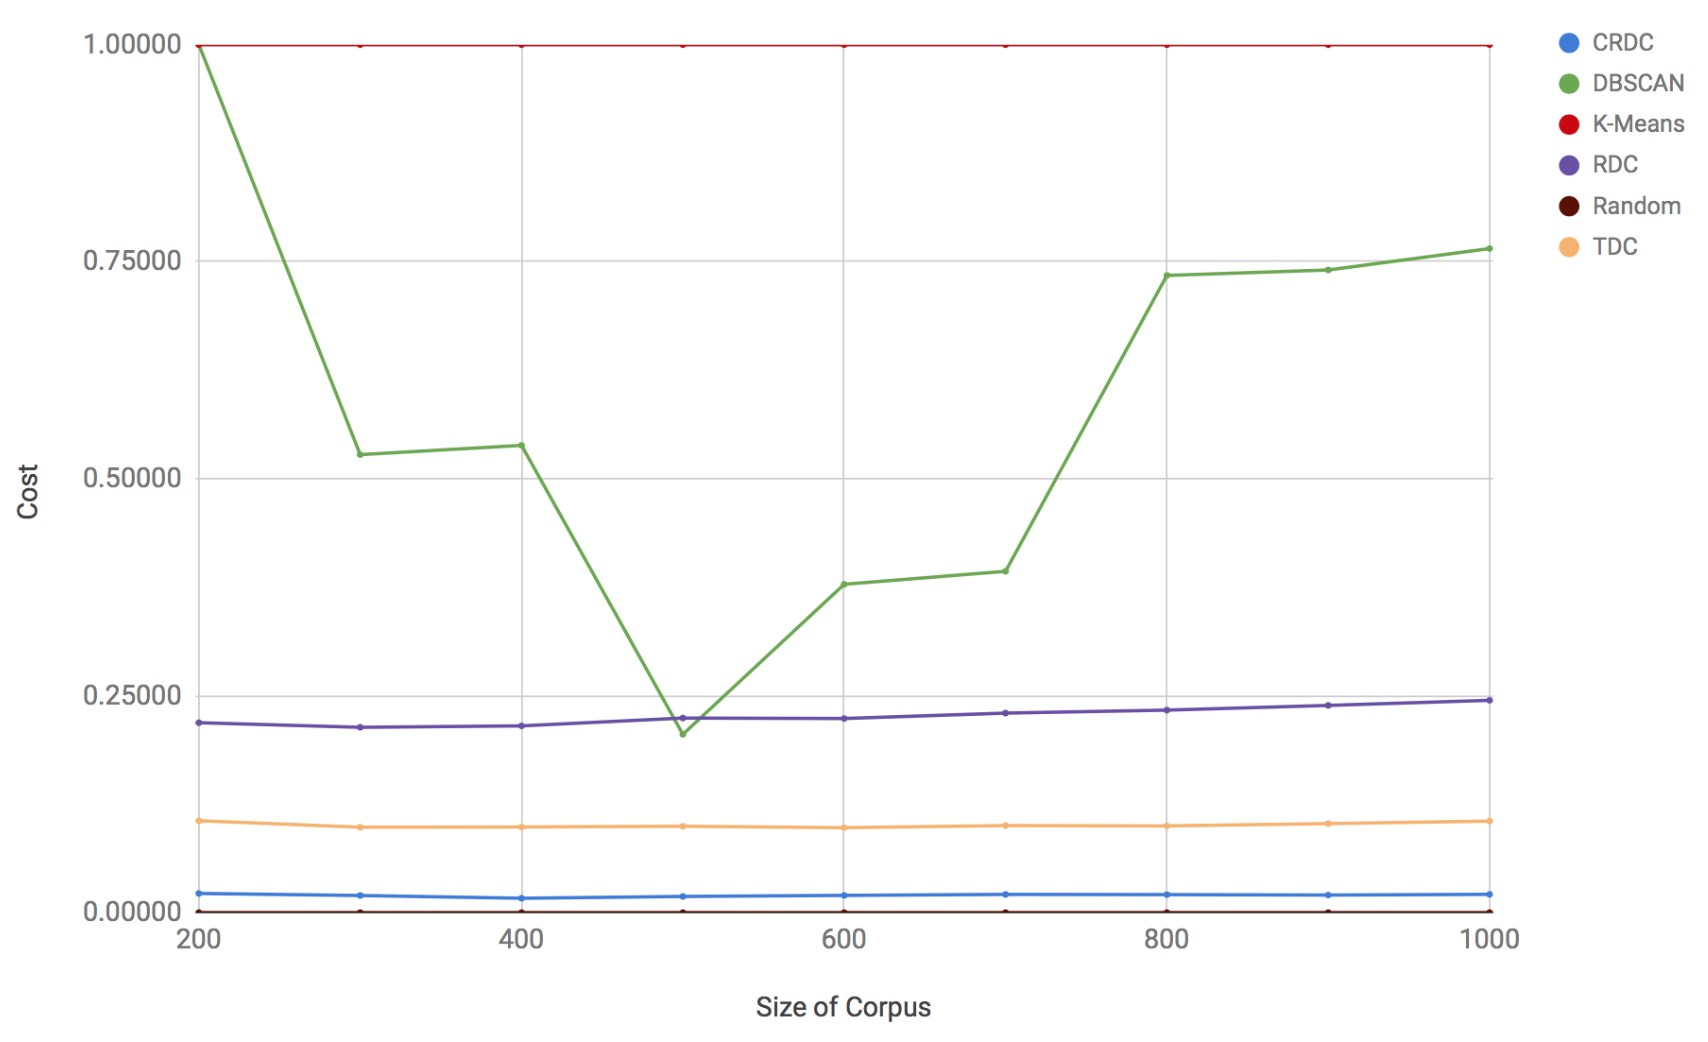
\includegraphics[scale=0.45]{costJS.png}
  \caption{Cost (JS-based) in AIES}
  \label{fig:costJS}
\end{figure}

\begin{figure}[!htb]\centering
  \center
  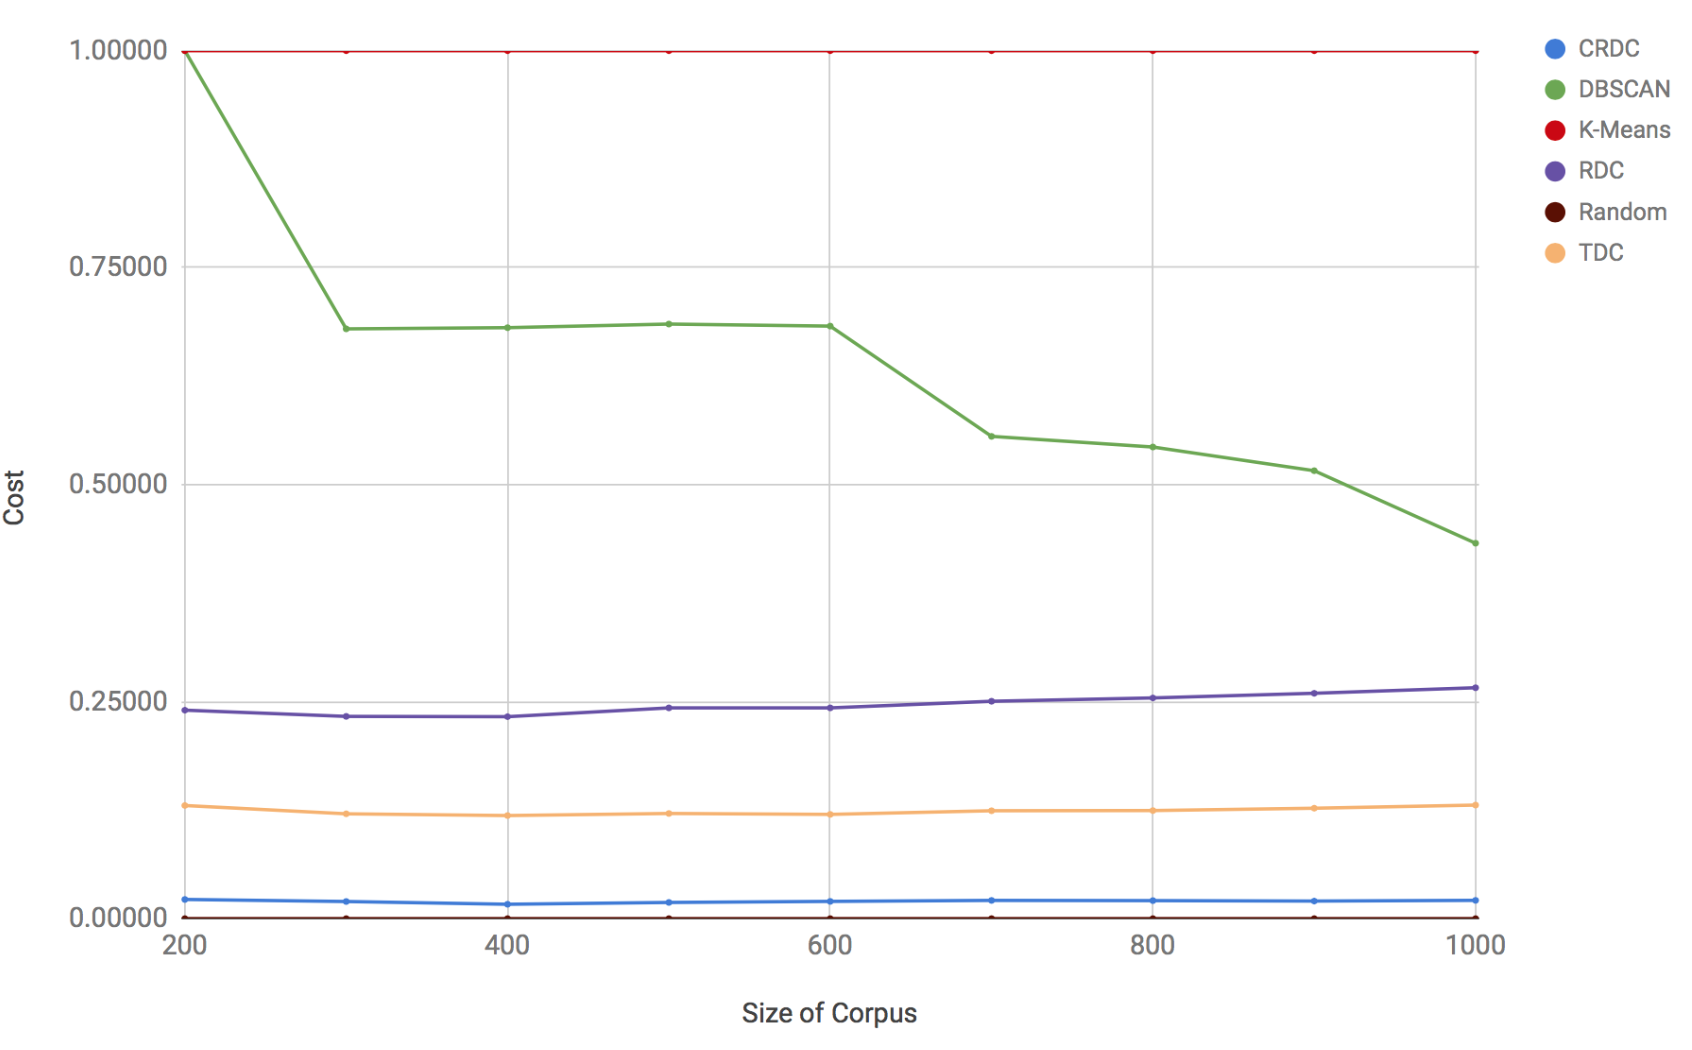
\includegraphics[scale=0.45]{costHe.png}
  \caption{Cost (He-based) in AIES}
  \label{fig:costHe}
\end{figure}

Finally, in terms of \textbf{\textit{efficiency}} (Figures ~\ref{fig:efficiencyJS}, ~\ref{fig:efficiencyHe}), regardless of the similarity measure used, the algorithm that yields the best performance according to the results obtained is \textit{CRDC}. Overall, \textit{CRDC} demonstrates a high accuracy classification and a lower cost by improving the performance offered by centroid-based or density-based approaches.

\begin{figure}[!htb]\centering
  \center
  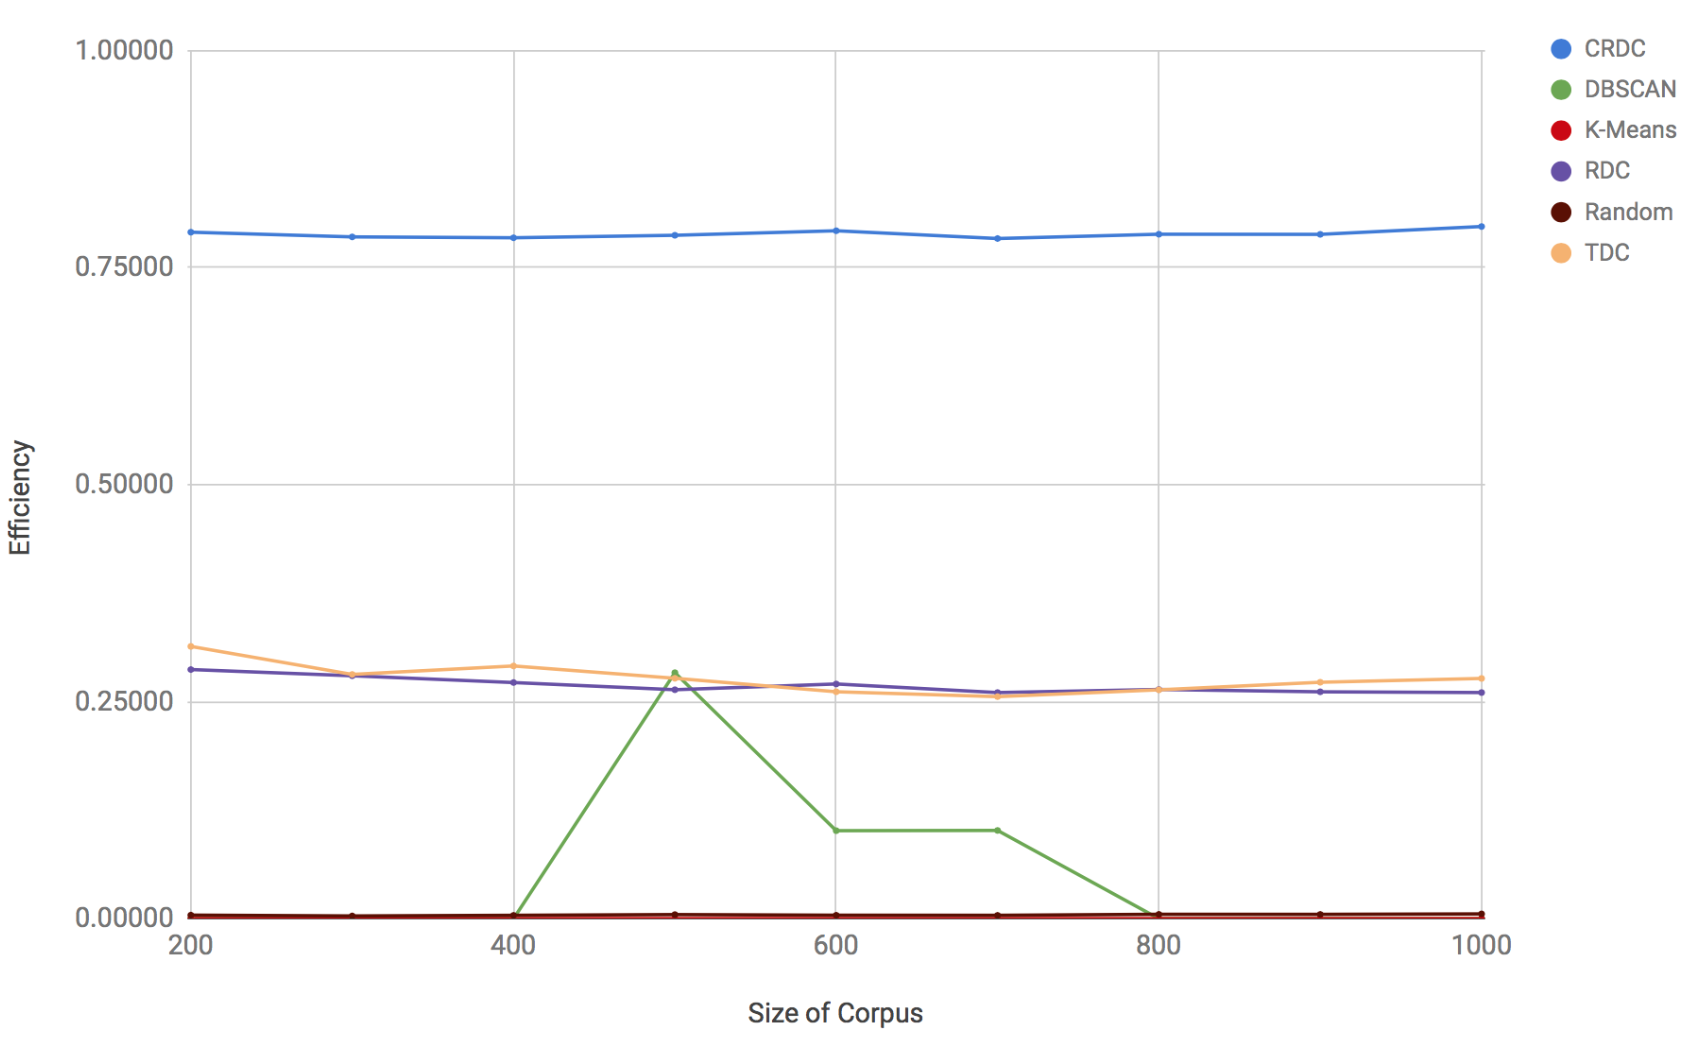
\includegraphics[scale=0.45]{efficiencyJS.png}
  \caption{Efficiency (JS-based) in AIES}
  \label{fig:efficiencyJS}
\end{figure}

\begin{figure}[!htb]\centering
  \center
  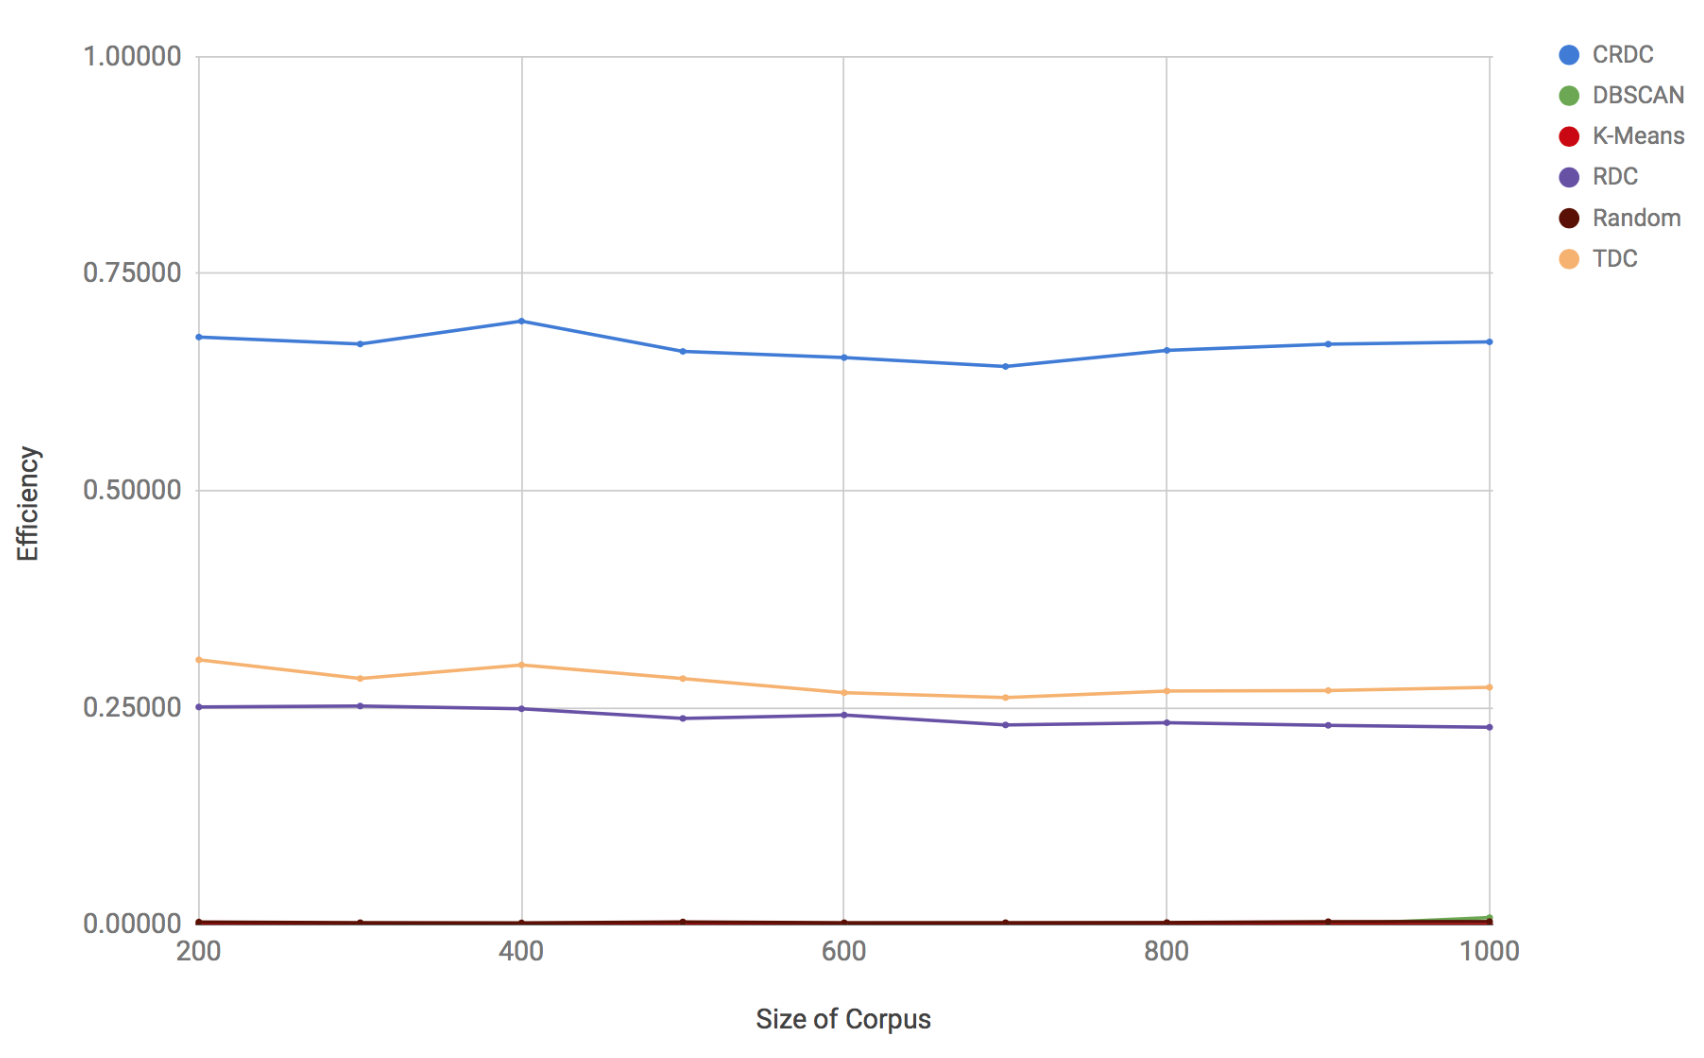
\includegraphics[scale=0.45]{efficiencyHe.png}
  \caption{Efficiency (He-based) in AIES}
  \label{fig:efficiencyHe}
\end{figure}

We have also created a synthetic dataset, DRM (Section ~\ref{sec:clustering-datasets}), composed of 1000 Dirichlet distributions with the same dimensions than topics in AIES: $k=44$. Unlike AIES, topic distributions have been randomly generated which imply that the similarity values are not so high: $min=0.06$, $mean=0.18$ and $max=0.61$. Following the same criteria than before (Section ~\ref{sec:clustering-threshold}), the similarity threshold is now fixed to 0.34 (Figure ~\ref{fig:similaritiesDRM}). Results \textbf{in terms of \textit{effectiveness}} (Figure ~\ref{fig:effectivenessDRMJS}) show a poor performance of the RDC and CRDC algorithms. The reason is that both are based on the fact that the highest weighted topics are shared between similar distributions. However, this condition is not satisfied when the similarity value between them is low.


\begin{figure}[!htb]\centering
  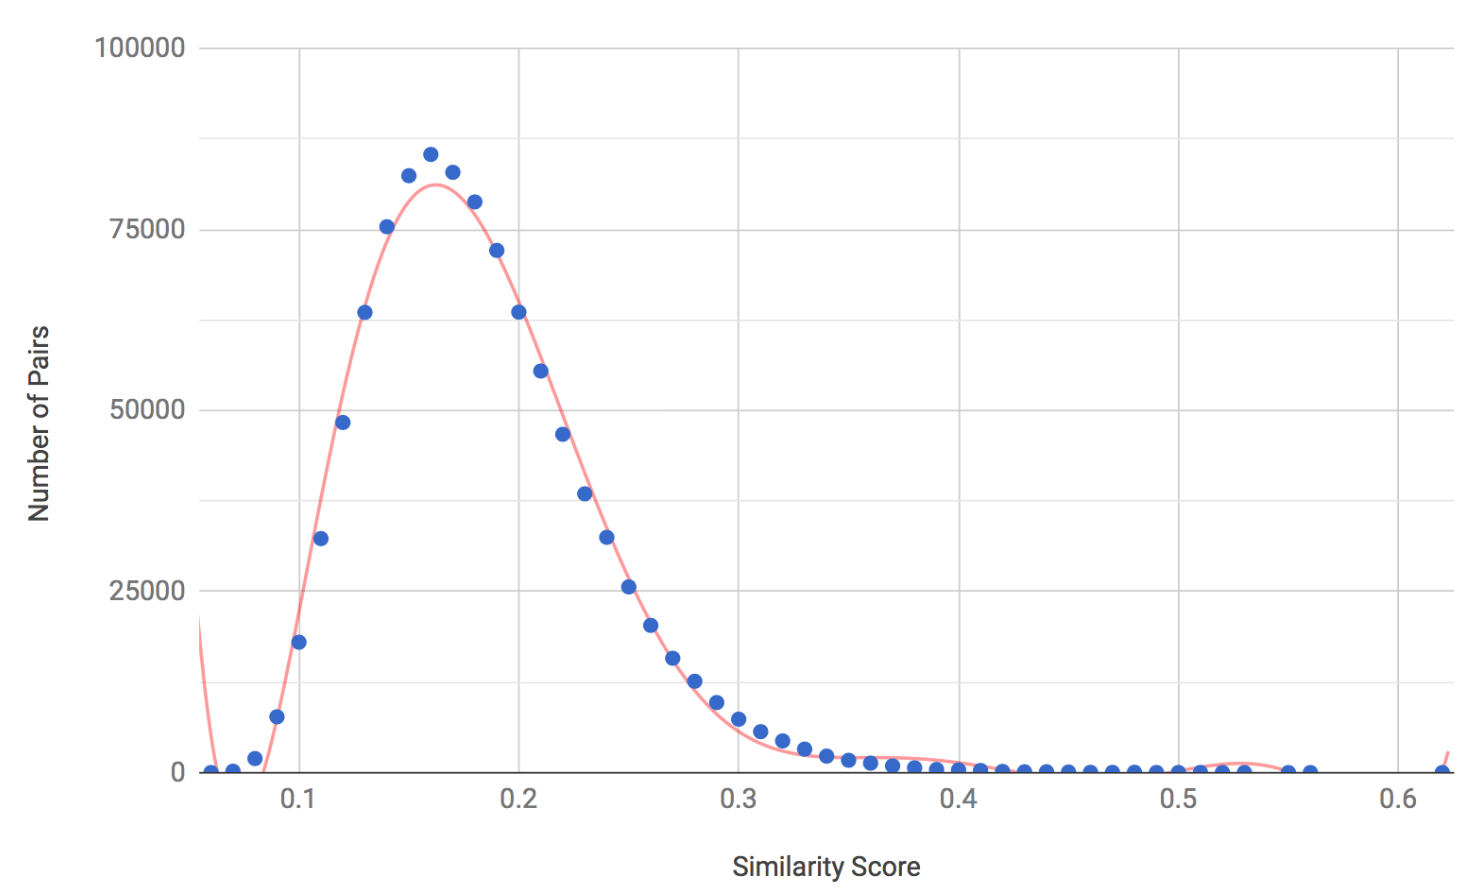
\includegraphics[scale=0.50]{similaritiesDRM.png}
  \caption{Similarity values grouped by frequency in DRM}
  \label{fig:similaritiesDRM}
\end{figure}


To confirm this behavior, we created a third dataset (DRM2) with the same size but with only 4 dimensions (4 topics). The goal is to achieve more similar distributions than in DRM even though they are also randomly generated. Since the similarity values range from $min=0.04$, $mean=0.34$ to $max=0.99$, the similarity threshold is now fixed to 0.66 (more details in section ~\ref{sec:clustering-threshold}). The results (Figure ~\ref{fig:effectivenessDRM2JS}) show an improvement in the accuracy of both the RDC and CRDC algorithms. Although scores are still not as high as for the AIES dataset, the increase compared to the DRM dataset shows that their \textit{precision} and \textit{recall} improve when the similarity threshold is higher. On the other hand, both the DBSCAN and TDC algorithms show similar behavior in both datasets, which means that their performance is not affected by the similarity threshold.

\subsection{Conclusion}
\label{sec:clustering-conclusion}

Processing a continuously growing collection of human generated documents requires techniques that divide the space into smaller regions containing potentially similar documents. Some algorithms in the literature tackle this problem from an unsupervised point of view, but they incur in high temporal costs and may not be suited for the domain being studied.

\begin{figure}[!htb]\centering
  \center
  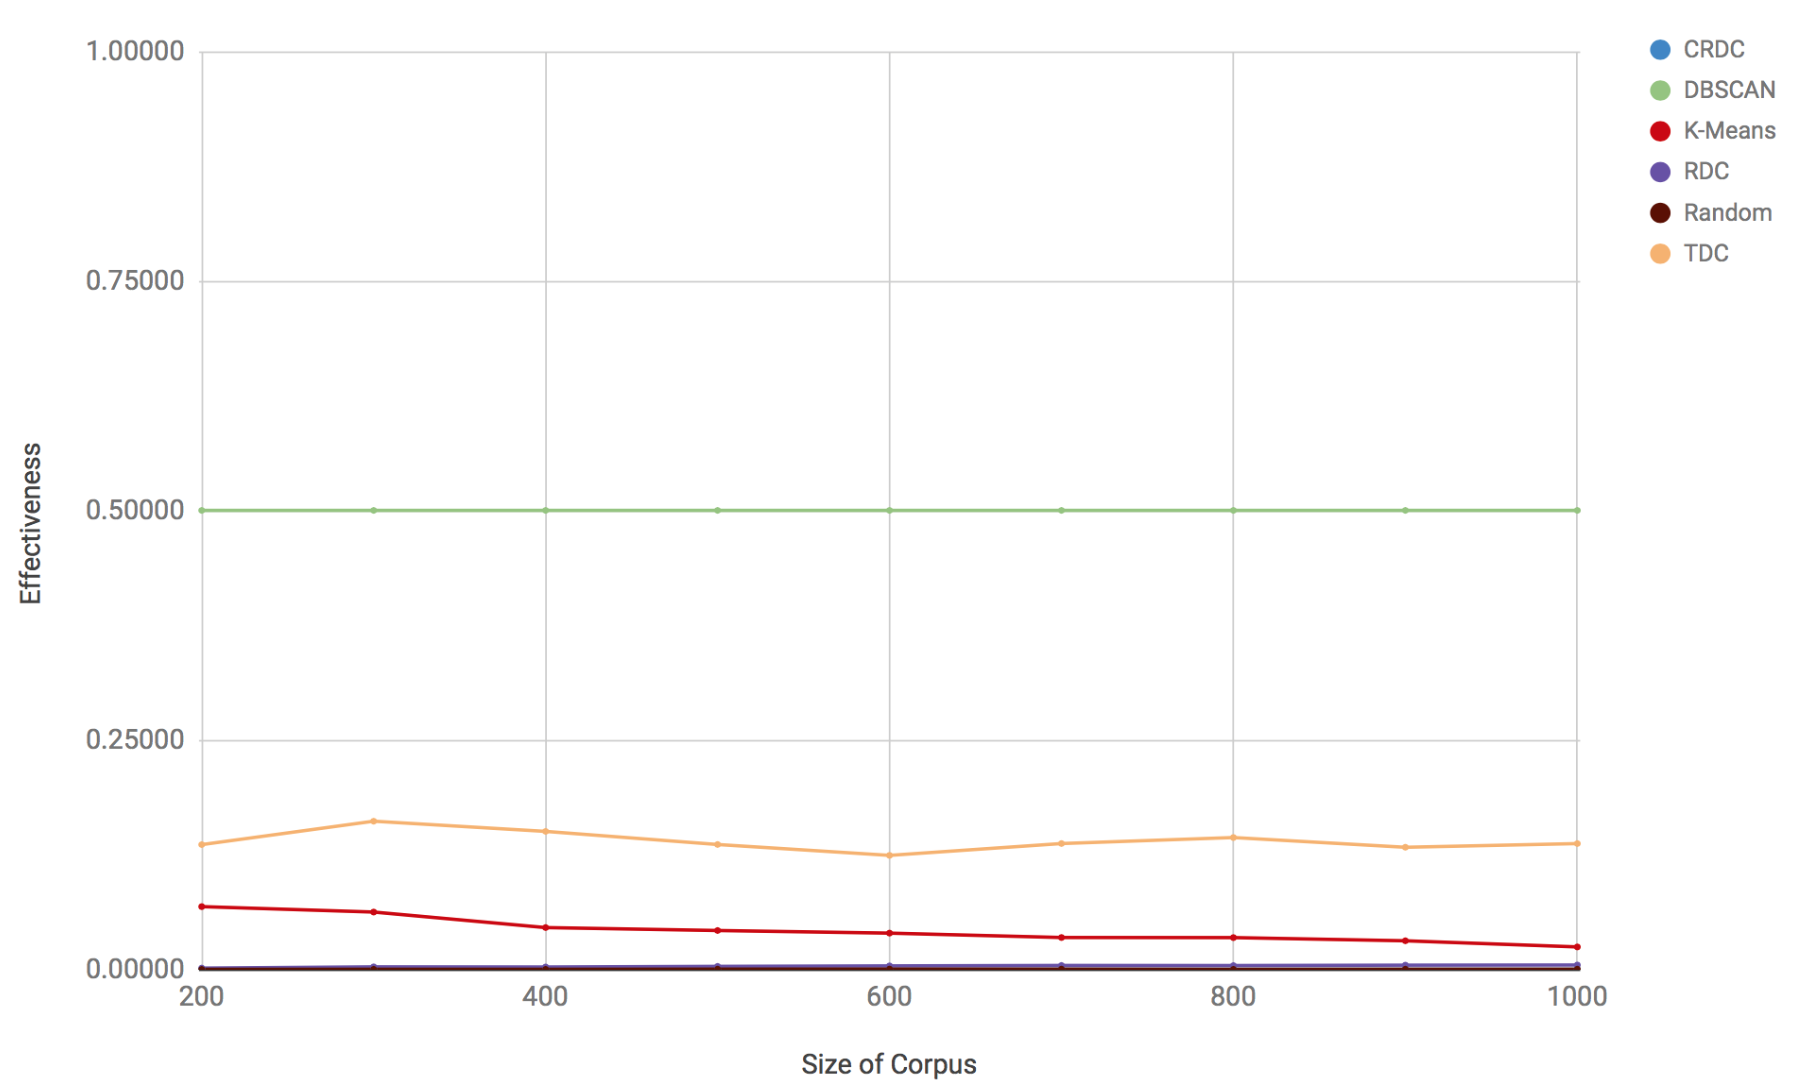
\includegraphics[scale=0.45]{effectivenessDRMJS.png}
  \caption{Effectiveness (JS based) in DRM}
  \label{fig:effectivenessDRMJS}
\end{figure}

\begin{figure}[!htb]\centering
  \center
  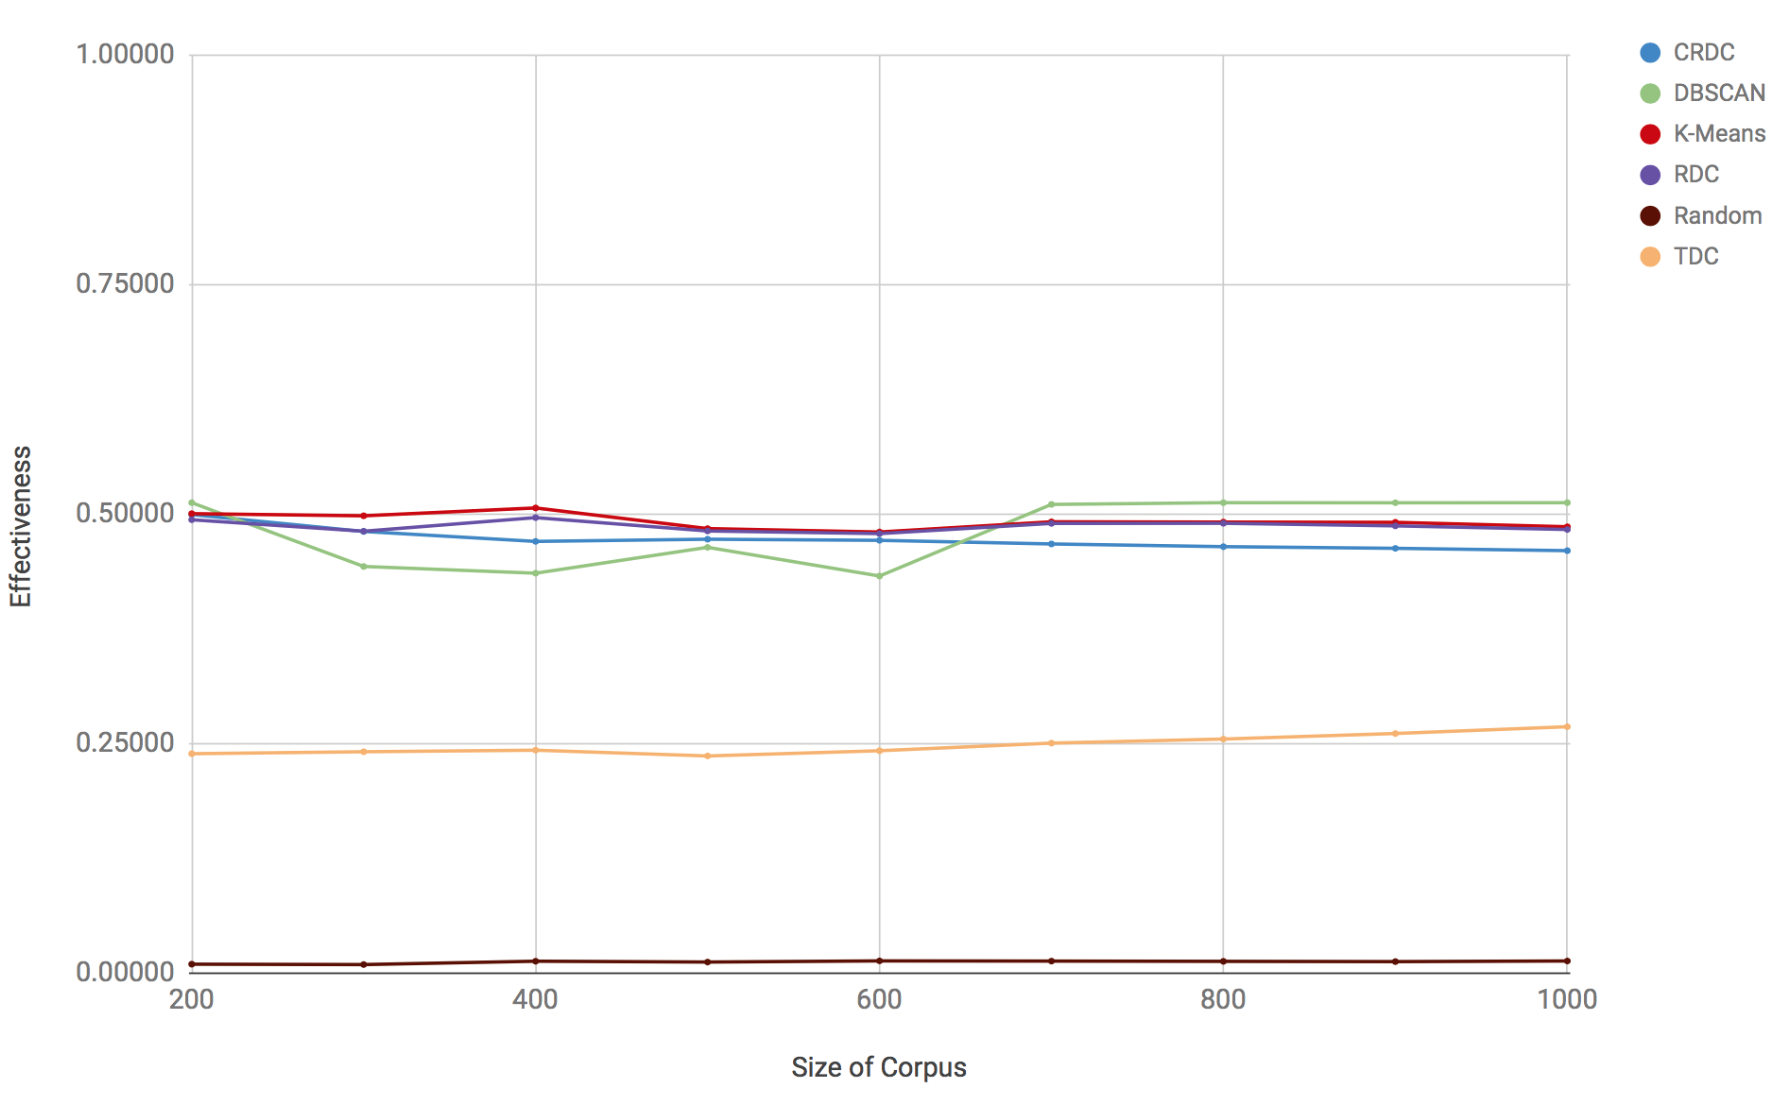
\includegraphics[scale=0.45]{effectivenessDRM2JS.png}
  \caption{Effectiveness (JS based) in DRM2}
  \label{fig:effectivenessDRM2JS}
\end{figure}


%Present solution.
Three novel unsupervised clustering algorithms, \textit{TDC}, \textit{RDC} and \textit{CRDC}, are described in this section relying on the distributions inferred from a topic modeling algorithm (LDA). They are presented as a means to identify a smaller set of documents where only the similarity function has to be computed. They leverage on the particular behavior of Dirichlet distributions describing topic distributions, where the highest weighted topics have a high influence on the rest of topics. This also means that given a topic distribution, the relations between their topic weights such as order or trends between them, are more important than the density values.

Although we initially thought that using only a fixed number of topics with higher weights of a topic distribution (\textit{RDC}), or taking into account only the trend changes between the weights of consecutive topics (\textit{TDC}), could be enough to classify similar topic distributions, the results obtained have shown that these properties are not sufficient. Results in terms of \textit{efficiency}, \textit{effectiveness} and \textit{cost} have been shown comparing the proposed algorithms with existing centroid-based and density-based clustering techniques. They reveal that obtaining the most representative topics of a topic distribution  by comparing the sum of their weights with respect to the rest (\textit{CRDC}) is a promising approach, which improves the \textit{efficiency} obtained by other centroid-based and density-based approaches. While \textit{K-Means} takes $O(n^k * \log{n})$ and \textit{DBSCAN} takes $O(n * \log{n})$ time to classify $n$ documents in a collection, the proposed algorithms only take linear time ($O(n)$) because they do not require any other data except their own topic distribution to assign it to a cluster.


\section{Summary}

In Section \ref{sec:topic-relations}, we have analyzed the representativeness of topics to describe texts, using the particular case of scientific articles. Our experiment with a corpus of research papers published in the \textit{Advances in Engineering Software} (AIES) journal shows that abstracts are not sufficiently representative to describe, by means of topics, the content of a paper. This behavior suggests that texts with greater vocabulary that emphasize key terms through repetition, favor topic-based representation. Therefore, if we want to construct a system that relates scientific articles, it would be better to use full texts rather than abstracts, as it is done by many more traditional techniques. This has a higher computational cost, for which systems like \textit{librAIry} behave sufficiently well.

Taking into account the relevance of topics to describe texts, we analyze in Section {\ref{sec:topic-clustering}} the behavior of topic distributions to calculate distances between documents using topic models with different dimensions. By using clustering techniques at the topic level, the most representative topics of a topic distribution are identified regardless of the number of dimensions that the model has. A topic-based representation is then proposed that covers the third research objective of this thesis (R03, \textit{define annotations based on topics that enable a semantic-aware exploration of the knowledge inside a corpus}). 

A new distance metric is also proposed that takes advantage of such representation to compare documents. Its performance is analyzed by automatically clustering the JRC-Acquis corpus according to EUROVOC categories. Tables \ref{tab:precisionHe}, \ref{tab:precisionJS}, \ref{tab:recallHe} and \ref{tab:recallJS} show results with high precision and recall in unsupervised classification tasks. This new way of relating documents from their most representative topics covers the fourth research objective of this thesis (R04, \textit{define a metric based on topic annotations that compares documents and facilitates their interpretation}). 

In order to perform the experiments, both the representation based on the most relevant topics and the distance metric based on these representations have been implemented in \textit{librAIry}. This partially covers the third and fourth technical objectives (T03, \textit{integrate the annotation method base on topic hierarchies into the topic model service}) (T04, \textit{create a system capable of finding similar document automatically}).